\documentclass[aspectratio=169, 10pt]{beamer}

% --- Tema e colori: sfondo nero ---
\usetheme{default}
\setbeamertemplate{navigation symbols}{}
\setbeamertemplate{footline}{%
    \hfill\textcolor{gray!50}{\insertframenumber}\hspace*{6pt}\vspace{4pt}%
}

% Sfondo nero globale
\setbeamercolor{background canvas}{bg=black}
% Testo bianco
\setbeamercolor{normal text}{fg=white}
\setbeamercolor{structure}{fg=white}
\setbeamercolor{itemize item}{fg=white}
\setbeamercolor{itemize subitem}{fg=white}
\setbeamercolor{enumerate item}{fg=white}
\setbeamercolor{block title}{fg=white, bg=white!15!black}
\setbeamercolor{block body}{fg=white, bg=white!8!black}
\setbeamercolor{block title alerted}{fg=white, bg=red!40!black}
\setbeamercolor{block body alerted}{fg=white, bg=red!10!black}
\setbeamertemplate{itemize item}{\textcolor{white}{$\bullet$}}

% --- Pacchetti ---
\usepackage[utf8]{inputenc}
\usepackage[T1]{fontenc}
\usepackage[italian]{babel}
\usepackage{amsmath, amssymb}
\usepackage{graphicx}
\usepackage{tikz}
\usetikzlibrary{shapes.geometric, arrows.meta, positioning, calc, shadows, decorations.pathreplacing}
\usepackage{booktabs}
\usepackage{xcolor}
\usepackage{colortbl}
\usepackage{pgfplots}
\pgfplotsset{compat=1.18}

% --- Percorsi immagini ---
\graphicspath{
    {../main/pictures/}
    {../main/pictures/cap2/}
    {../main/pictures/cap5/}
    {../main/pictures/cap6/}
    {../summary/}
}

% --- Comando titolo rainbow (colori del prisma) ---
\newcommand{\rainbowtitle}[1]{%
    \begin{tikzpicture}
        \node[inner sep=0pt, outer sep=0pt] (text) {%
            \phantom{\Large\bfseries #1}%
        };
        \shade[left color=red, right color=violet,
               middle color=green!80!yellow]
            (text.south west) rectangle (text.north east);
        \node[inner sep=0pt, outer sep=0pt] at (text.center) {%
            \Large\bfseries #1%
        };
    \end{tikzpicture}%
}

% Ridefinisci il frametitle per usare colori rainbow
\setbeamertemplate{frametitle}{%
    \vspace{0.3cm}
    \begin{tikzpicture}
        \node[anchor=west, inner sep=0pt] (title) at (0,0) {%
            \phantom{\Large\bfseries\insertframetitle}%
        };
        \shade[left color=red, middle color=yellow!80!green, right color=violet]
            ([yshift=-1pt]title.south west) rectangle ([yshift=1pt]title.south east);
        \node[anchor=west, inner sep=0pt, text=white] at (0,0) {%
            \Large\bfseries\insertframetitle%
        };
    \end{tikzpicture}%
    \vspace{0.1cm}
}

% --- Metadati ---
\title[PRISMA]{PRISMA}
\subtitle{Projection of Representations for Interpretability\\via Sparse Monosemantic Autoencoders}
\author{Edoardo Tedesco}
\institute{Corso di Laurea Magistrale in Fisica\\Universit\`a degli Studi di Milano}


\begin{document}

% ============================================================
% TITOLO
% ============================================================
\begin{frame}[plain]
    % --- Sfondo prisma semi-trasparente ---
    \begin{tikzpicture}[remember picture, overlay]
        \node[opacity=0.3, inner sep=0pt] at (current page.center) {%
            
\includegraphics[width=\paperwidth]{pictures/prism.jpg}%
        };
    \end{tikzpicture}

    \begin{center}
        \vspace{0.3cm}
        % Logo universita invertito (bianco su trasparente)
        
\includegraphics[height=1.6cm]{pictures/logo_unimi_white.png}

        \vspace{0.5cm}

        % Titolo PRISMA con effetto rainbow
        \begin{tikzpicture}
            \node[inner sep=0pt] (t) {\phantom{\fontsize{36}{40}\selectfont\bfseries PRISMA}};
            \shade[left color=red, right color=violet, middle color=green!80!yellow]
                (t.south west) rectangle (t.north east);
            \node[inner sep=0pt, text=white] at (t.center) {\fontsize{36}{40}\selectfont\bfseries PRISMA};
        \end{tikzpicture}

        \vspace{0.1cm}

        % Linea rainbow sottile
        \begin{tikzpicture}
            \shade[left color=red, middle color=yellow!80!green, right color=violet]
                (0,0) rectangle (10,0.03);
        \end{tikzpicture}

        \vspace{0.3cm}
        % Acronimo con iniziali colorate
        {\small\color{gray!70}
            \textcolor{red}{\textbf{P}}rojection of
            \textcolor{orange}{\textbf{R}}epresentations for
            \textcolor{yellow}{\textbf{I}}nterpretability via
            \textcolor{green}{\textbf{S}}parse
            \textcolor{cyan}{\textbf{M}}onosemantic
            \textcolor{violet}{\textbf{A}}utoencoders}

        \vspace{0.6cm}

        {\small\color{white!70}\textsc{Disentanglement e scomposizione  in feature monosemantiche delle rappresentazioni latenti nei LLM\\}}
        \vspace{0.2cm}
        {\color{gray} Edoardo Tedesco}

        \vspace{0.2cm}
        {\small\color{gray!60} Corso di Laurea Magistrale in Fisica\\
        Universit\`a degli Studi di Milano}

        \vspace{0.3cm}
        {\footnotesize\color{gray!50}
        Relatore esterno: Prof. Mirko Cesarini \quad$\cdot$\quad Relatore interno: Prof. Marco Gherardi}

        \vspace{0.2cm}
        
    \end{center}
\end{frame}

% ============================================================
% SLIDE 1 — L'inizio: 30 novembre 2022
% ============================================================
\begin{frame}{30 novembre 2022}
    \vspace{-0.2cm}
    \begin{columns}[T]

        % --- Colonna sinistra: SUPER NOVA GRANDE ---
        \begin{column}{0.45\textwidth}
            \centering
            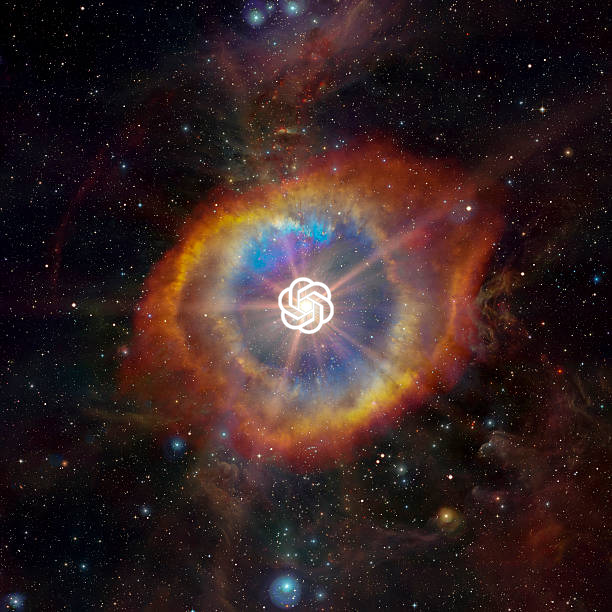
\includegraphics[
                width=\textwidth,
                height=7cm,
                keepaspectratio
            ]{pictures/supernova_chatgpt_explosion.png}
        \end{column}

        % --- Colonna destra ---
        \begin{column}{0.53\textwidth}
            \centering

            % Introducing ChatGPT + Board affiancati
            \begin{columns}[T]
                \begin{column}{0.55\textwidth}
                    \centering
                    
\includegraphics[
                        width=\textwidth,
                        height=2cm,
                        keepaspectratio
                    ]{pictures/introducing_chatgpt.jpeg}
                \end{column}
                \begin{column}{0.42\textwidth}
                    \centering
                    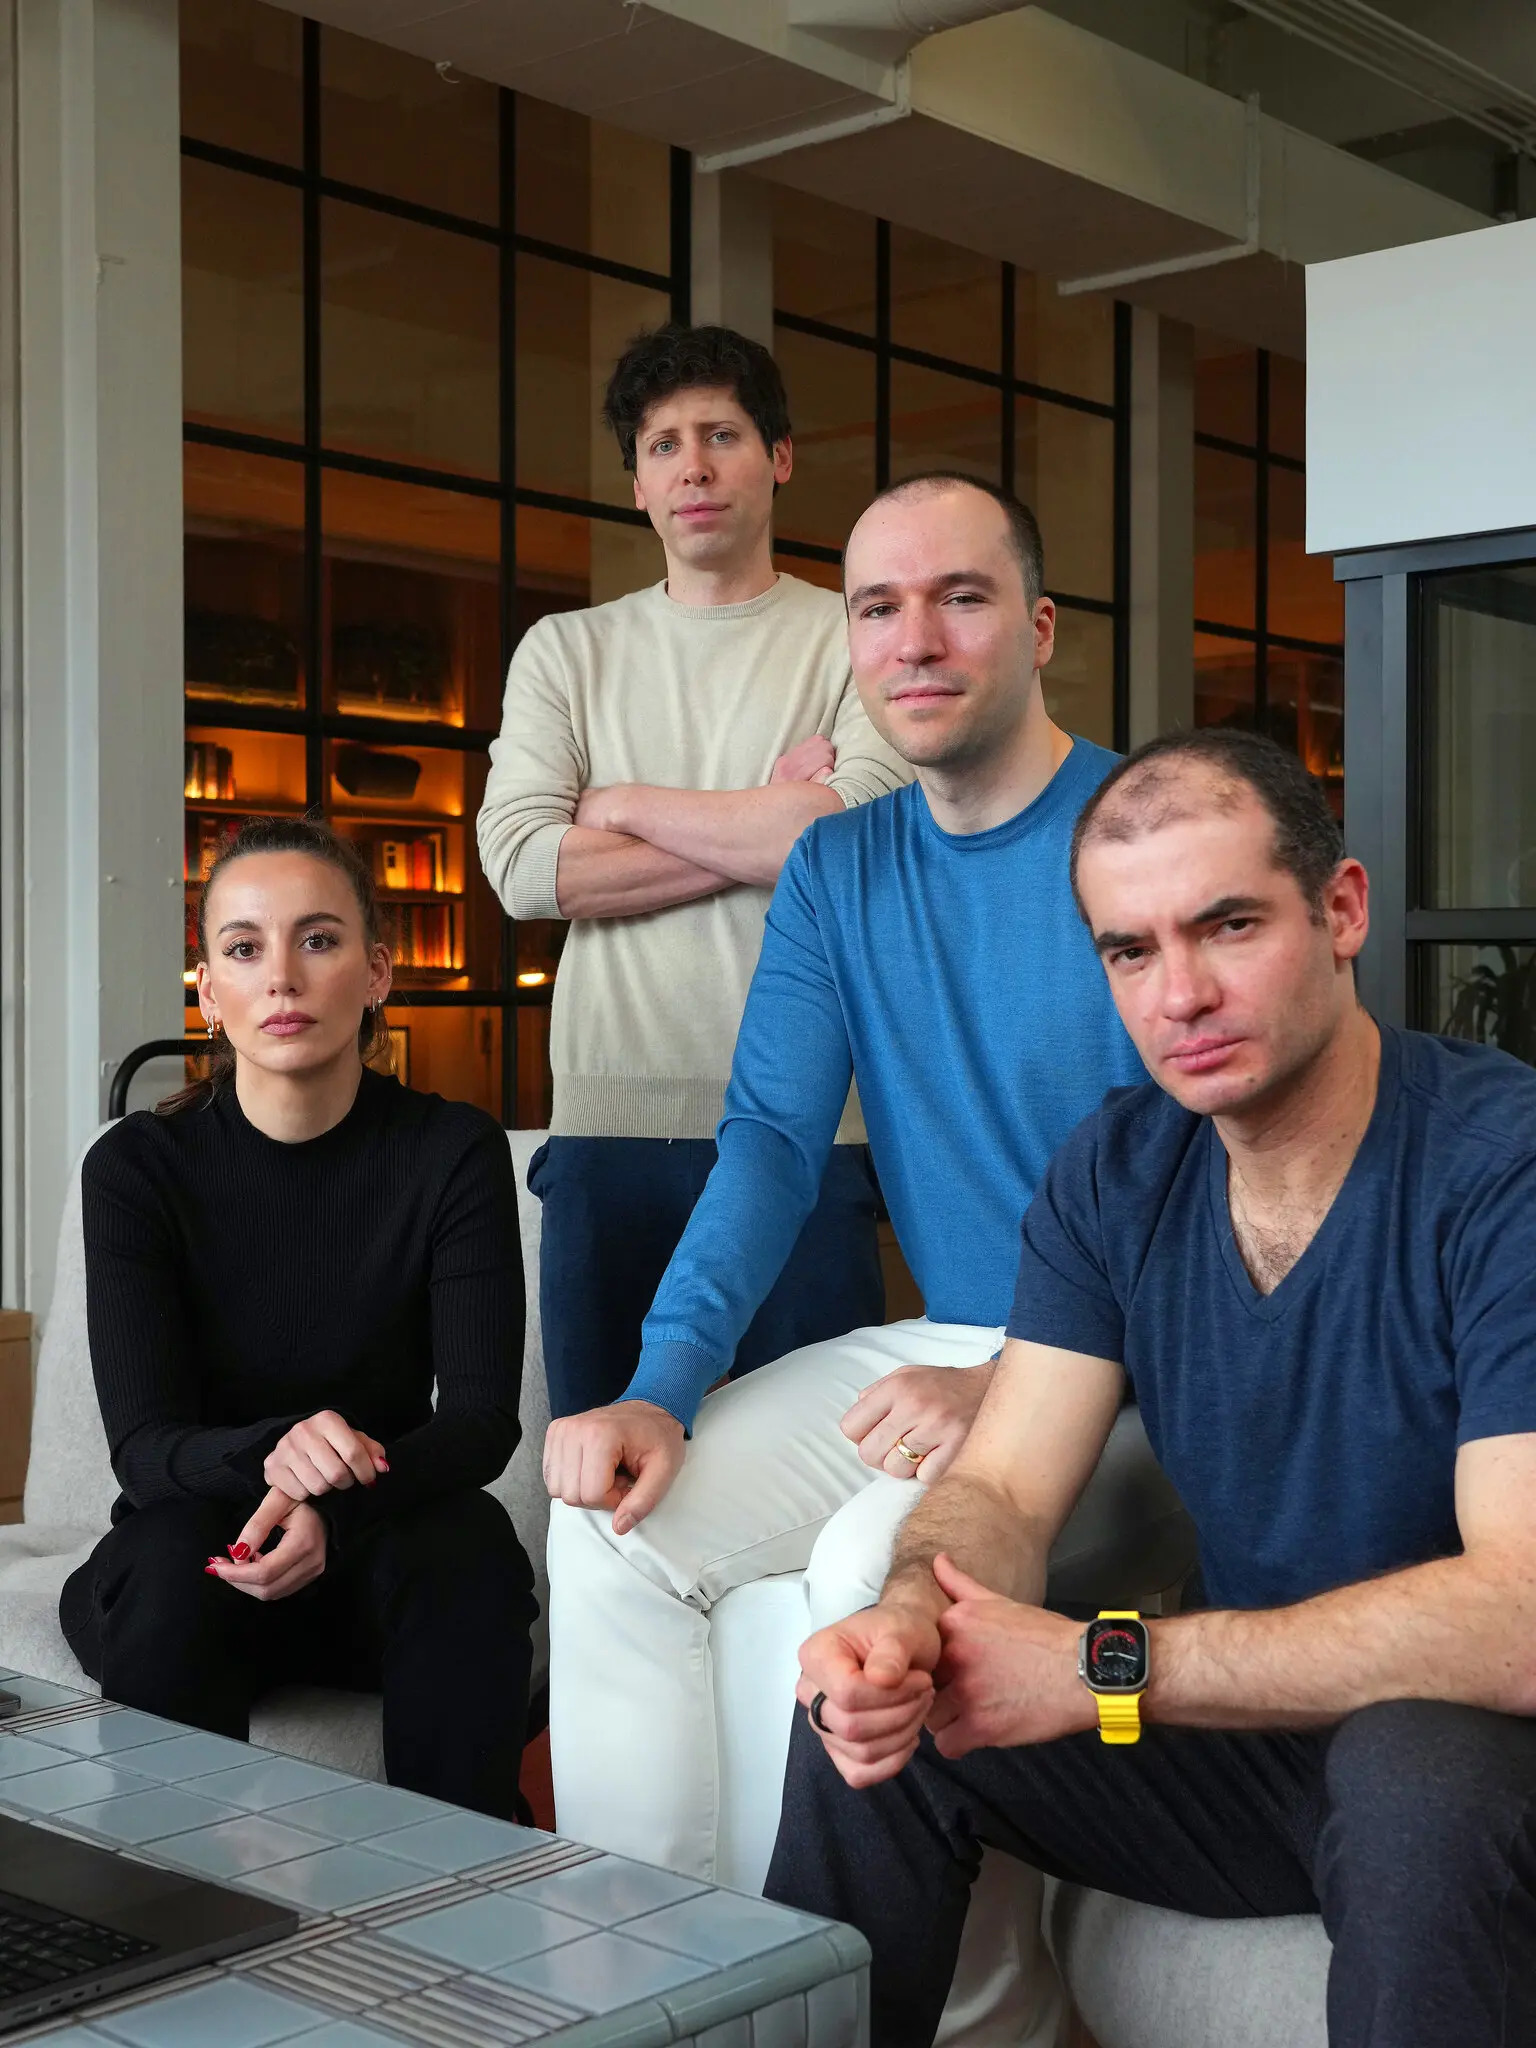
\includegraphics[
                        width=\textwidth,
                        height=2cm,
                        keepaspectratio
                    ]{pictures/openai_board.jpg}
                \end{column}
            \end{columns}

            \vspace{0.15cm}

            % --- Google Trends Plot (largo) ---
            \begin{tikzpicture}
                \begin{axis}[
                    width=\textwidth,
                    height=4.5cm,
                    axis background/.style={fill=black},
                    axis line style={white},
                    tick style={white},
                    ticklabel style={color=white, font=\scriptsize},
                    xlabel style={color=gray!70, font=\small},
                    ylabel style={color=gray!70, font=\small},
                    title style={color=white, font=\small\bfseries},
                    title={Google Trends: ``Artificial Intelligence''},
                    xmin=0, xmax=70,
                    ymin=0, ymax=110,
                    xtick={0, 12, 24, 36, 48, 60, 70},
                    xticklabels={2020, 2021, 2022, 2023, 2024, 2025, },
                    grid=major,
                    grid style={gray!20},
                ]
                    \addplot[fill=cyan!30!black, draw=none, forget plot]
                        table[x=x, y=y] {data/ai_trends.dat}
                        \closedcycle;
                    \addplot[cyan!80, very thick]
                        table[x=x, y=y] {data/ai_trends.dat};
                    \draw[red!70, thick, dashed] (axis cs:36,0) -- (axis cs:36,110);
                    \node[red!70, font=\tiny, anchor=south west] at (axis cs:37,85) {ChatGPT};
                \end{axis}
            \end{tikzpicture}

        \end{column}

    \end{columns}
\end{frame}


% ============================================================
% SLIDE 2 — La domanda da fisico
% ============================================================
\begin{frame}{La domanda da fisico}
    \begin{columns}
        \begin{column}{0.55\textwidth}
            Il linguaggio contiene \textbf{semantica}.

            \vspace{0.4cm}
            Le macchine hanno appreso delle \textbf{leggi} per manipolarlo.

            \vspace{0.4cm}
            Possiamo mettere il linguaggio sotto le \textbf{lenti della fisica}?

            \vspace{0.4cm}
            Le macchine possono aiutarci a trovare \textbf{leggi della semantica}?
        \end{column}
        \begin{column}{0.4\textwidth}
            \centering
            \begin{tikzpicture}[scale=0.9]
                % Assi
                \draw[->, thick, white] (0,0) -- (4,0) node[below, midway, font=\scriptsize, white] {Capacit\`a predittiva};
                \draw[->, thick, white] (0,0) -- (0,3.5) node[above, font=\scriptsize, white] {Interpretabilit\`a};

                % Regione fisica
                \fill[blue!40, rounded corners, opacity=0.6] (0.2,2.0) rectangle (1.5,3.0);
                \node[align=center, font=\tiny, white] at (0.85,2.5) {Leggi\\fisiche};

                % Regione reti neurali
                \fill[red!40, rounded corners, opacity=0.6] (2.5,0.3) rectangle (3.7,1.3);
                \node[align=center, font=\tiny, white] at (3.1,0.8) {Reti\\neurali};

                % Punto ideale
                \fill[green!70] (3.1,2.7) circle (2.5pt);
                \node[anchor=west, font=\tiny, white] at (3.25,2.7) {\textbf{Ideale}};

                % Frecce ortogonali
                \draw[->, dashed, thick, green!70] (3.1,1.3) -- (3.1,2.55);
                \draw[->, dashed, thick, green!70] (1.5,2.7) -- (2.95,2.7);
            \end{tikzpicture}
        \end{column}
    \end{columns}
\end{frame}

% ============================================================
% SLIDE 3 — Feynman e il metodo
% ============================================================
\begin{frame}{L’Autoencoder}
    \begin{columns}
        \begin{column}{0.45\textwidth}
            \centering
            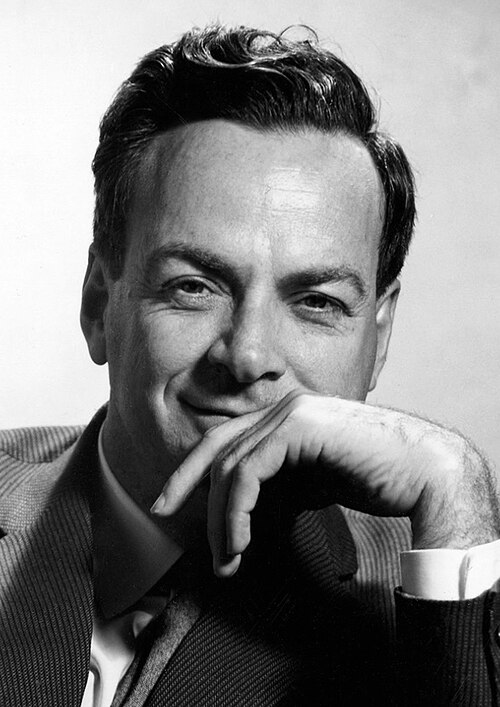
\includegraphics[width=0.75\textwidth]{cap2/Richard_Feynman_Nobel.jpg}

            \vspace{0.2cm}
            {\footnotesize Richard P. Feynman\\Premio Nobel per la Fisica, 1965}
        \end{column}
        \begin{column}{0.5\textwidth}
            \begin{block}{}
                \Large\itshape
                ``What I cannot build,\\I do not understand.''
            \end{block}

            \vspace{0.5cm}
            Hai capito davvero qualcosa solo quando sei capace di \textbf{aprirlo}, vedere com'\`e fatto dentro, e \textbf{ricostruirlo}.
        \end{column}
    \end{columns}
\end{frame}

% ============================================================
% SLIDE 4 — L'Autoencoder
% ============================================================
\begin{frame}{L'Autoencoder}
    \centering
    \begin{tikzpicture}[
        scale=0.95,
        transform shape,
        node distance=1.2cm,
        every node/.style={font=\small, text=white}
    ]
        \node[draw=gray!50, rectangle, minimum height=3cm, minimum width=0.8cm, fill=gray!80] (input) {Input $\mathbf{x}$};
        \node[draw=gray!50, trapezium, trapezium angle=70, shape border rotate=270, minimum height=1.6cm, fill=blue!40!black, right=of input] (enc) {Encoder};
        \node[draw=gray!50, rectangle, minimum height=1cm, minimum width=0.8cm, fill=red!40!black, right=of enc] (latent) {$n<d$};
        \node[draw=gray!50, trapezium, trapezium angle=70, shape border rotate=90, minimum height=1.6cm, fill=blue!40!black, right=of latent] (dec) {Decoder};
        \node[draw=gray!50, rectangle, minimum height=3cm, minimum width=0.8cm, fill=gray!80, right=of dec] (output) {Output $\hat{\mathbf{x}}$};

        \draw[->, thick, white] (input) -- (enc);
        \draw[->, thick, white] (enc) -- (latent);
        \draw[->, thick, white] (latent) -- (dec);
        \draw[->, thick, white] (dec) -- (output);
    \end{tikzpicture}

    \vspace{0.3cm}
\begin{columns}[T]
        \begin{column}{0.48\textwidth}
            \textbf{Encoder:} \quad $f: \mathbb{R}^d \to \mathbb{R}^n$
        \end{column}
        \begin{column}{0.48\textwidth}
            \textbf{Decoder:} \quad $g: \mathbb{R}^n \to \mathbb{R}^d$
        \end{column}
    \end{columns}

    \vspace{0.2cm}
    \begin{itemize}
        \item Si forza la macchina a \textbf{ricostruire} i dati di input
        \item A partire da un numero di variabili \textbf{inferiore} ($n < d$)
        \item La macchina \`e costretta a \textbf{capire} cosa \`e essenziale
    \end{itemize}

    \vspace{0.3cm}
    \centering
    $\mathcal{L} = \|\mathbf{x} - \hat{\mathbf{x}}\|^2 = \|\mathbf{x} - g(f(\mathbf{x}))\|^2$

\end{frame}

% ============================================================
% SLIDE — Autoencoder: compressione senza semantica
% ============================================================
\begin{frame}{Autoencoder}
    \centering
    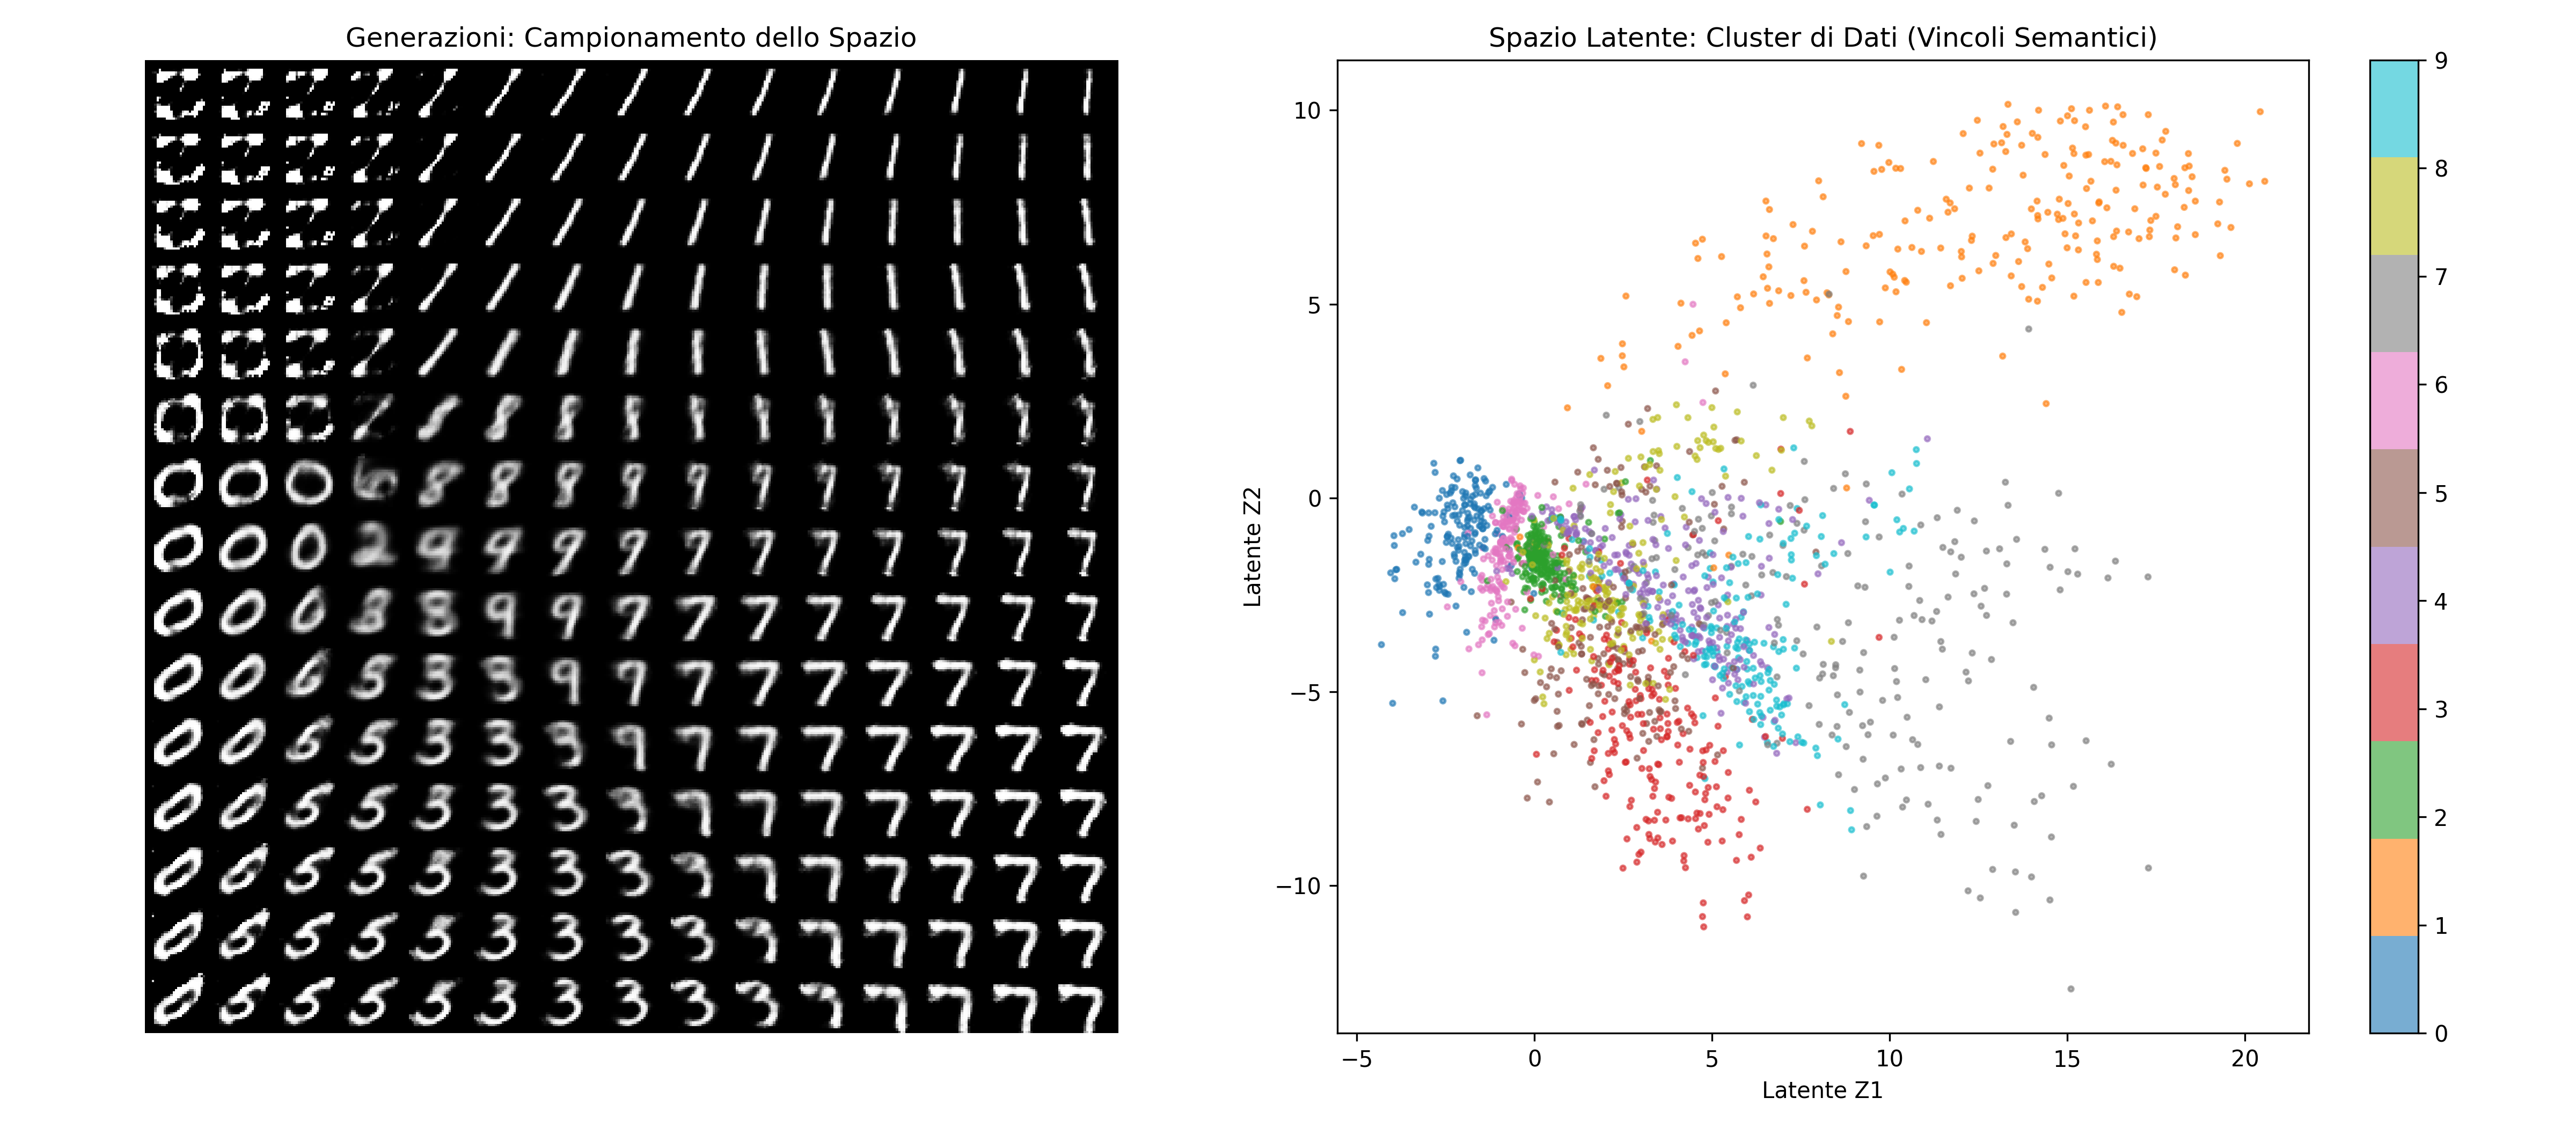
\includegraphics[width=\textwidth, height=0.85\textheight, keepaspectratio]{pictures/ae_no_semantics.png}
\end{frame}
% ============================================================
% SLIDE 5 — Significanti e significati
% ============================================================
\begin{frame}{Significanti e significati}
    \centering
    \begin{tikzpicture}[scale=0.75]
        % Insieme dei Significanti
        \draw[thick, draw=blue!50, fill=blue!15!black] (-4,0) ellipse (2cm and 2.5cm);
        \node[anchor=south, font=\small\bfseries, white] at (-4,2.5) {Significanti ($\mathcal{S}$)};
        \node[white] (s1) at (-4,1.2) {``cane''};
        \node[white] (s2) at (-4,0.3) {``dog''};
        \node[white] (s3) at (-4,-0.7) {``medico''};
        \node[white] (s4) at (-4,-1.6) {``dottore''};

        % Insieme dei Significati
        \draw[thick, draw=green!50, fill=green!10!black] (4,0) ellipse (2cm and 2.5cm);
        \node[anchor=south, font=\small\bfseries, white] at (4,2.5) {Significati ($\mathbb{R}^d$)};

        % Punti
        \filldraw[green!70] (3.5,0.8) circle (2pt) node[anchor=west, white] (v1) {\small $\vec{v}_{\text{canine}}$};
        \filldraw[green!70] (3.5,-1.0) circle (2pt) node[anchor=west, white] (v2) {\small $\vec{v}_{\text{medical}}$};

        % Frecce
        \draw[->, >=stealth, thick, gray!50] (s1) to [bend left=10] (v1);
        \draw[->, >=stealth, thick, gray!50] (s2) to [bend right=10] (v1);
        \draw[->, >=stealth, thick, gray!50] (s3) to [bend left=10] (v2);
        \draw[->, >=stealth, thick, gray!50] (s4) to [bend right=10] (v2);

        \node[font=\large, white] at (0,0.8) {$f: \mathcal{S} \to \mathbb{R}^d$};
    \end{tikzpicture}

    \vspace{0.3cm}
    Le macchine non parlano la nostra lingua: parlano la \textbf{lingua dei numeri}.

    \vspace{0.1cm}
    Gli \textbf{embeddings} traducono parole $\to$ vettori.
\end{frame}

% ============================================================
% SLIDE 6 — L'ipotesi distribuzionale
% ============================================================
\begin{frame}{L'ipotesi distribuzionale}
    \begin{block}{}
        \centering
        \Large \textit{Parole con significati simili si trovano in contesti simili.}
    \end{block}

    \vspace{0.3cm}
    \centering
    \small
    \arrayrulecolor{gray!50}
    \begin{tabular}{lcccc}
        \toprule
        & \textbf{As You Like It} & \textbf{Twelfth Night} & \textbf{Julius Caesar} & \textbf{Henry V} \\
        \midrule
        battle & 1   & 0  & 7  & 13 \\
        good   & 114 & 80 & 62 & 89 \\
        fool   & 36  & 58 & 1  & 4  \\
        wit    & 20  & 15 & 2  & 3  \\
        \bottomrule
    \end{tabular}

    \vspace{0.3cm}
    Parole con distribuzioni simili sui documenti $\Rightarrow$ \textbf{vettori simili}
\end{frame}

% ============================================================
% SLIDE 7 — Il problema del contesto
% ============================================================
\begin{frame}{Il problema del contesto}
    Gli embeddings basati sulla sola occorrenza sono \textbf{statici}.

    \vspace{0.3cm}
    Ma le parole cambiano significato in base al contesto:

    \vspace{0.4cm}
    \centering
    \begin{tikzpicture}
        % Frase 1
        \node[font=\normalsize, white, anchor=west] at (0, 1.2) {``Vado a \textbf{pesca} al lago''};
        \node[font=\small, green!60, anchor=west] at (9, 1.2) {$\to$ \textit{fishing}};

        % Frase 2
        \node[font=\normalsize, white, anchor=west] at (0, 0) {``Ho comprato una \textbf{pesca} al mercato''};
        \node[font=\small, orange!60, anchor=west] at (9, 0) {$\to$ \textit{peach}};

        % Separatore
        \draw[gray!40, dashed] (0, -0.6) -- (12, -0.6);

        % Conclusione
        \node[font=\normalsize, white, anchor=west] at (0, -1.3) {Stessa parola, \textbf{stesso vettore} $\to$ non va bene!};
    \end{tikzpicture}

    \vspace{0.5cm}
    Serve un'inferenza \textbf{dinamica}: il vettore deve dipendere dal \textbf{contesto}.
\end{frame}

% ============================================================
% SLIDE 7b — Gli assi del linguaggio
% ============================================================
\begin{frame}{Gli assi del linguaggio}
    \begin{columns}[T]
        \begin{column}{0.30\textwidth}
            \centering
            \vspace{0.2cm}
            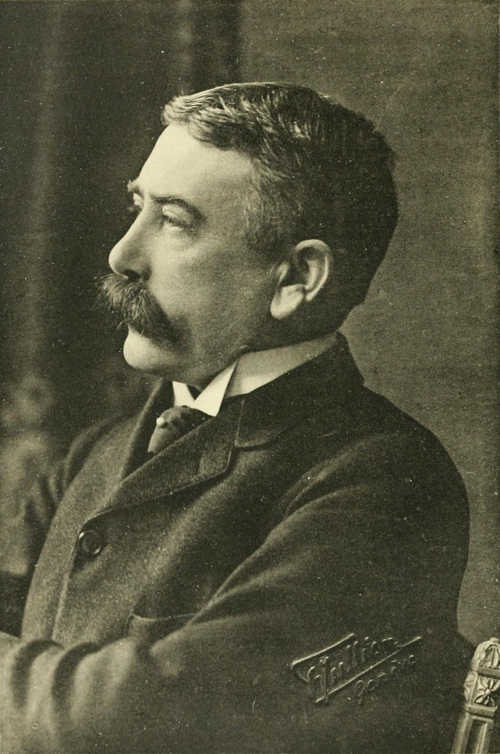
\includegraphics[width=0.85\textwidth]{pictures/Ferdinand_de_Saussure_by_Jullien.png}

            \vspace{0.2cm}
            {\footnotesize Ferdinand de Saussure}
        \end{column}
        \begin{column}{0.65\textwidth}
            Il linguaggio si articola lungo due assi fondamentali:

            \vspace{0.2cm}
            \centering
            \begin{tikzpicture}[scale=0.65]
                % Assi
                \draw[->, thick, blue!50] (-4.2, 0) -- (5.5, 0);
                \draw[->, thick, red!50] (0, -2.8) -- (0, 3.5);

                % Parola centrale
                \node[draw=yellow!60, fill=yellow!25!black, rounded corners=3pt, inner sep=6pt, font=\large\bfseries, text=yellow!90] at (0,0) {mangia};

                % Sintagmatico (orizzontale)
                \node[font=\normalsize, white, fill=black, inner sep=2pt] at (-2.5, 0) {Il gatto};
                \node[font=\normalsize, white, fill=black, inner sep=2pt] at (3.0, 0) {la mela};

                % Paradigmatico (verticale)
                \node[font=\small\itshape, gray!70, fill=black, inner sep=1pt] at (0, 1.4) {rincorre};
                \node[font=\small\itshape, gray!70, fill=black, inner sep=1pt] at (0, 2.3) {osserva};
                \node[font=\small\itshape, gray!70, fill=black, inner sep=1pt] at (0, -1.4) {divora};
                \node[font=\small\itshape, gray!70, fill=black, inner sep=1pt] at (0, -2.3) {gusta};

                % Labels
                \node[font=\tiny\bfseries, blue!60, anchor=north] at (4.5, -0.3) {Asse Sintagmatico};
                \node[font=\tiny, blue!50, anchor=north] at (4.5, -0.8) {``quale parola segue?''};
                \node[font=\tiny\bfseries, red!60, anchor=west] at (0.4, 3.3) {Asse Paradigmatico};
                \node[font=\tiny, red!50, anchor=west] at (0.4, 2.9) {``cosa potrei mettere al posto di...?''};
            \end{tikzpicture}

            \vspace{0.3cm}
            \flushleft
            Aumentare il \textbf{sintagma} milgiora il \textbf{paradigma}. Serve più contesto. 
        \end{column}
    \end{columns}
\end{frame}

% ============================================================
% SLIDE 7c — I paper fondamentali
% ============================================================
\begin{frame}{Dai Transformers a BERT}
    \centering
    \vspace{0.3cm}
    \begin{columns}[c]
        \begin{column}{0.45\textwidth}
            \centering
            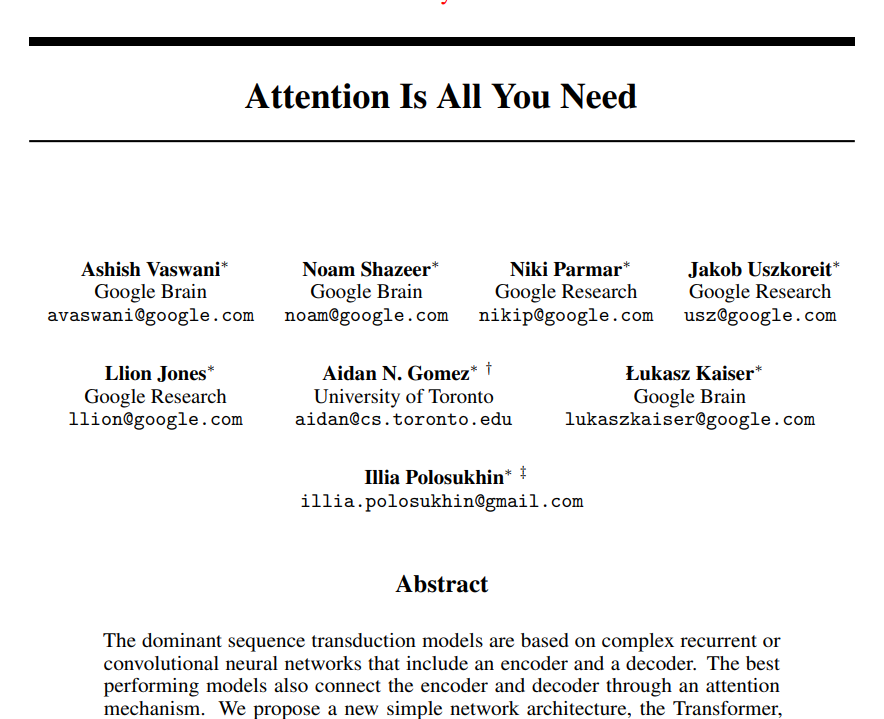
\includegraphics[width=0.85\textwidth, height=5.5cm, keepaspectratio]{pictures/attention_is_all_you_need.png}

            \vspace{0.2cm}
            {\footnotesize Vaswani et al., 2017}
        \end{column}
        \begin{column}{0.05\textwidth}
            \centering
            {\Large $\Rightarrow$}
        \end{column}
        \begin{column}{0.45\textwidth}
            \centering
            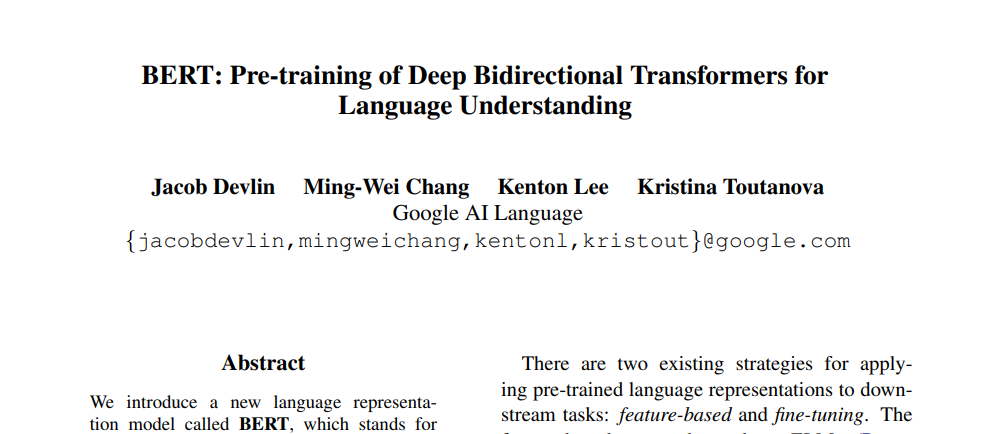
\includegraphics[width=0.85\textwidth, height=5.5cm, keepaspectratio]{pictures/bert_2018.png}

            \vspace{0.2cm}
            {\footnotesize Devlin et al., 2018}
        \end{column}
    \end{columns}
\end{frame}

% ============================================================
% SLIDE 8 — BERT e i Masked Language Models
% ============================================================
\begin{frame}{BERT e i Masked Language Models}
    \textbf{B}idirectional \textbf{E}ncoder \textbf{R}epresentations from \textbf{T}ransformers

    \vspace{0.3cm}
    Per \textbf{predire la parola mancante}, la macchina \`e costretta a costruirsi una \textbf{rappresentazione interna del mondo}.

    \vspace{0.4cm}
    \centering
    \begin{tikzpicture}
        % Parole
        \node[draw=gray!50, rounded corners, fill=blue!50!black, minimum width=1.4cm, minimum height=0.8cm, font=\small, text=white] (w0) at (0, 0) {Il};
        \node[draw=gray!50, rounded corners, fill=blue!50!black, minimum width=1.4cm, minimum height=0.8cm, font=\small, text=white] (w1) at (2.4, 0) {gatto};
        \node[draw=red!60, rounded corners, fill=red!40!black, minimum width=1.4cm, minimum height=0.8cm, font=\small\bfseries, text=white] (w2) at (4.8, 0) {[MASK]};
        \node[draw=gray!50, rounded corners, fill=blue!50!black, minimum width=1.4cm, minimum height=0.8cm, font=\small, text=white] (w3) at (7.2, 0) {la};
        \node[draw=gray!50, rounded corners, fill=blue!50!black, minimum width=1.4cm, minimum height=0.8cm, font=\small, text=white] (w4) at (9.6, 0) {mela};

        % Attenzione bidirezionale: frecce da [MASK] sotto i box, archi verso il basso
        \draw[->, thick, orange!60, opacity=0.5] (w2.south) to[bend left=30] node[below, font=\tiny, orange!80] {0.05} (w0.south);
        \draw[->, thick, orange!80, opacity=0.8] (w2.south) to[bend left=20] node[below, font=\tiny, orange!80] {0.35} (w1.south);
        \draw[->, thick, orange!60, opacity=0.5] (w2.south) to[bend right=20] node[below, font=\tiny, orange!80] {0.10} (w3.south);
        \draw[->, thick, orange!90] (w2.south) to[bend right=30] node[below, font=\tiny, orange!80] {0.50} (w4.south);

        % Freccia bidirezionale etichetta
        \draw[<->, thick, cyan!60] (-0.7, -1.8) -- (10.3, -1.8);
        \node[font=\scriptsize, cyan!60] at (4.8, -2.2) {attenzione \textbf{bidirezionale}};

        % Output: encoder produce embedding
        \draw[->, very thick, green!60] (4.8, -2.6) -- (4.8, -3.2);
        \node[font=\scriptsize, green!60] at (6.3, -2.9) {Encoder};

        % Embedding
        \node[draw=green!50, rounded corners, fill=green!15!black, minimum width=3cm, minimum height=0.7cm, font=\small, text=white] at (4.8, -3.8) {$\mathbf{e}_i \in \mathbb{R}^{768}$};
    \end{tikzpicture}

    \vspace{0.3cm}
    BERT \`e un \textbf{Encoder}: per ogni token produce un embedding in $\mathbb{R}^{768}$.
\end{frame}

% ============================================================
% SLIDE 9 — Il problema: 768 dimensioni e Superposition
% ============================================================
\begin{frame}{Il problema: L'ipotesi della Superposition (Anthropic)}
    \begin{columns}[T]
        \begin{column}{0.32\textwidth}
            \centering
            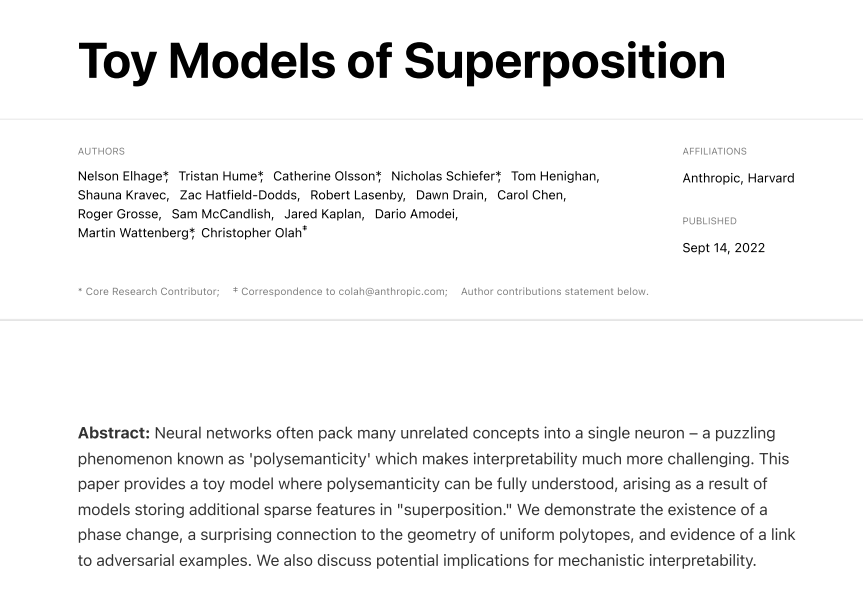
\includegraphics[width=\textwidth, height=5cm, keepaspectratio]{pictures/superposition.png}

            \vspace{0.2cm}
            {\tiny Elhage et al., Anthropic 2022}
        \end{column}
        \begin{column}{0.63\textwidth}
            Le 768 dimensioni di BERT \textbf{non sono interpretabili}.

            \vspace{0.2cm}
            ``\textit{meccanica quantistica}'' raramente si trova nel contesto di ``\textit{torta al cioccolato}''.

            \vspace{0.2cm}
            Le macchine fanno una cosa intelligentissima: conservano l'attivazione di un neurone per \textbf{molteplici significati}.

            \vspace{0.1cm}
            {\small\color{gray!60} ``Tanto questi due non si accenderanno mai insieme.''}

            \vspace{0.2cm}
            \centering
            \begin{tikzpicture}[scale=1.4]
                \draw[->, thick, gray!50] (-1.1,0) -- (1.3,0) node[right, font=\tiny, gray!60] {$d_1$};
                \draw[->, thick, gray!50] (0,-0.9) -- (0,1.3) node[above, font=\tiny, gray!60] {$d_2$};

                \draw[->, ultra thick, orange!80] (0,0) -- (1,0);
                \node[anchor=north, font=\tiny\bfseries, orange!80] at (1, -0.06) {$\mathbf{w}_{\text{torta}}$};

                \draw[->, ultra thick, cyan!80] (0,0) -- ({cos(120)},{sin(120)});
                \node[anchor=south east, font=\tiny\bfseries, cyan!80] at ({cos(120)-0.05},{sin(120)+0.03}) {$\mathbf{w}_{\text{quant}}$};

                \draw[->, ultra thick, green!70] (0,0) -- ({cos(240)},{sin(240)});
                \node[anchor=north east, font=\tiny\bfseries, green!70] at ({cos(240)-0.05},{sin(240)-0.03}) {$\mathbf{w}_{\text{ricetta}}$};

                \draw[red!60, thick] (0.25,0) arc (0:120:0.25);
                \node[red!60, font=\tiny] at (0.18, 0.32) {$120^\circ$};
            \end{tikzpicture}
        \end{column}
    \end{columns}
\end{frame}

% ============================================================
% SLIDE 10 — PRISMA
% ============================================================
\begin{frame}{PRISMA}
    \centering
    \begin{tikzpicture}[scale=1.1]
        % Prisma (triangolo)
        \coordinate (A) at (0, 0);
        \coordinate (B) at (3, 0);
        \coordinate (C) at (1.5, 2.6);

        \fill[blue!15!black] (A) -- (B) -- (C) -- cycle;
        \draw[thick, blue!40] (A) -- (B) -- (C) -- cycle;

        % Raggio incidente
        \draw[->, ultra thick, gray!50] (-2.5, 1.3) -- (0.75, 1.3);
        \node[above, font=\small, white] at (-1.2, 1.35) {Embedding denso $\mathbf{x}$};

        % Raggi rifratti
        \draw[->, thick, red!80] (2.25, 0.9) -- (5, 0.0);
        \draw[->, thick, orange!90] (2.25, 0.9) -- (5, 0.5);
        \draw[->, thick, yellow!85!black] (2.25, 0.9) -- (5, 1.0);
        \draw[->, thick, green!70!black] (2.25, 0.9) -- (5, 1.5);
        \draw[->, thick, blue!70] (2.25, 0.9) -- (5, 2.0);
        \draw[->, thick, violet!80] (2.25, 0.9) -- (5, 2.5);

        % Etichette feature (tema: meccanica quantistica + torta al cioccolato)
        \node[right, font=\scriptsize, red!80] at (5, 0.0) {$h_1$: funzione d'onda};
        \node[right, font=\scriptsize, orange!90] at (5, 0.5) {$h_2$: cioccolato fondente};
        \node[right, font=\scriptsize, yellow!80] at (5, 1.0) {$h_3$: principio di indeterminazione};
        \node[right, font=\scriptsize, green!70] at (5, 1.5) {$h_4$: ricetta dolce};
        \node[right, font=\scriptsize, blue!70] at (5, 2.0) {$h_5$: entanglement quantistico};
        \node[right, font=\scriptsize, violet!80] at (5, 2.5) {$h_6$: forno a 180\textdegree{}C};

        % Etichetta prisma
        \node[font=\small\bfseries, white] at (1.5, -0.5) {PRISMA};
    \end{tikzpicture}

    \vspace{0.2cm}
    {\small\textbf{P}rojection of \textbf{R}epresentations for \textbf{I}nterpretability via \textbf{S}parse \textbf{M}onosemantic \textbf{A}utoencoders}
    

    \vspace{0.2cm}
    {\small Scomporre l'embedding denso nelle sue \textbf{feature monosemantiche}: concetti atomici interpretabili.}
\end{frame}


% ============================================================
% SLIDE 12 — Come funziona PRISMA: lo Sparse Autoencoder
% ============================================================
\begin{frame}{Come funziona PRISMA: lo Sparse Autoencoder}
    \centering
    \begin{tikzpicture}[scale=0.8, transform shape, every node/.style={text=white}]
        \node[draw=gray!50, rectangle, minimum height=2.5cm, minimum width=0.7cm, fill=gray!60] (input) at (0,0) {$x \in \mathbb{R}^{d}$};
        \node[draw=gray!50, trapezium, trapezium angle=70, shape border rotate=90, minimum height=2cm, fill=green!25!black] (enc) at (3.0,0) {Encoder};
        \node[draw=gray!50, rectangle, minimum height=5cm, minimum width=1.8cm, fill=red!20!black] (latent) at (6,0) {};
        \node[font=\small] at (6, 0) {$h \in \mathbb{R}^{n}$};
        % Sparse activation dots
        \fill[green!70] (6, 2.0) circle (3pt);
        \fill[gray!40] (6, 1.5) circle (3pt);
        \fill[gray!40] (6, 1.0) circle (3pt);
        \fill[green!70] (6, 0.5) circle (3pt);
        \fill[gray!40] (6, -0.5) circle (3pt);
        \fill[gray!40] (6, -1.0) circle (3pt);
        \fill[green!70] (6, -1.5) circle (3pt);
        \fill[gray!40] (6, -2.0) circle (3pt);
        \node[font=\small, gray!60] at (6, -3.0) {$n \gg d$};
        \node[draw=gray!50, trapezium, trapezium angle=70, shape border rotate=270, minimum height=2cm, fill=green!25!black] (dec) at (9.0,0) {Decoder};
        \node[draw=gray!50, rectangle, minimum height=2.5cm, minimum width=0.7cm, fill=gray!60] (output) at (12,0) {$\hat{x} \approx x$};
        \draw[->, thick, white] (input) -- (enc);
        \draw[->, thick, white] (enc) -- (latent);
        \draw[->, thick, white] (latent) -- (dec);
        \draw[->, thick, white] (dec) -- (output);
    \end{tikzpicture}

    \vspace{0.3cm}
    \begin{columns}[T]
        \begin{column}{0.48\textwidth}
            \textbf{Encoder} (non lineare):
            \vspace{-0.1cm}
            \[
                h = f_\theta(x) = \sigma(W_e\, x + b_e)
            \]
        \end{column}
        \begin{column}{0.48\textwidth}
            \textbf{Decoder} (lineare):
            \vspace{-0.1cm}
            \[
                \hat{x} = g_\phi(h) = W_d\, h + b_d
            \]
        \end{column}
    \end{columns}

    \vspace{0.1cm}
    \textbf{Loss:} \quad $\mathcal{L} = \frac{1}{d}\|x - \hat{x}\|_2^2 + \lambda\, \mathcal{L}_{\text{sparse}}(h)$
\end{frame}
% ============================================================
% SLIDE 12b — Il vincolo di sparsit\`a e la rappresentazione latente
% ============================================================
\begin{frame}{Il vincolo di sparsit\`a}
    \begin{columns}[T]
        \begin{column}{0.55\textwidth}
            Perch\'e \textbf{Top-K} e non regolarizzazione $L_1$?

            \vspace{0.3cm}
            La penalizzazione $L_1$ causa \textbf{shrinkage}: le attivazioni vengono sistematicamente ridotte rispetto al loro valore reale, portando a rappresentazioni sub-ottimali.

            \vspace{0.3cm}
            Il vincolo \textbf{Top-K} mantiene le $k$ attivazioni pi\`u grandi \textbf{al loro valore esatto}, azzerando le restanti.

            \vspace{0.3cm}
            {\small\color{gray!60} O'Neill et al., \textit{Disentangling Dense Embeddings with Sparse Autoencoders}, 2024.}
        \end{column}
        \begin{column}{0.42\textwidth}
            \centering
            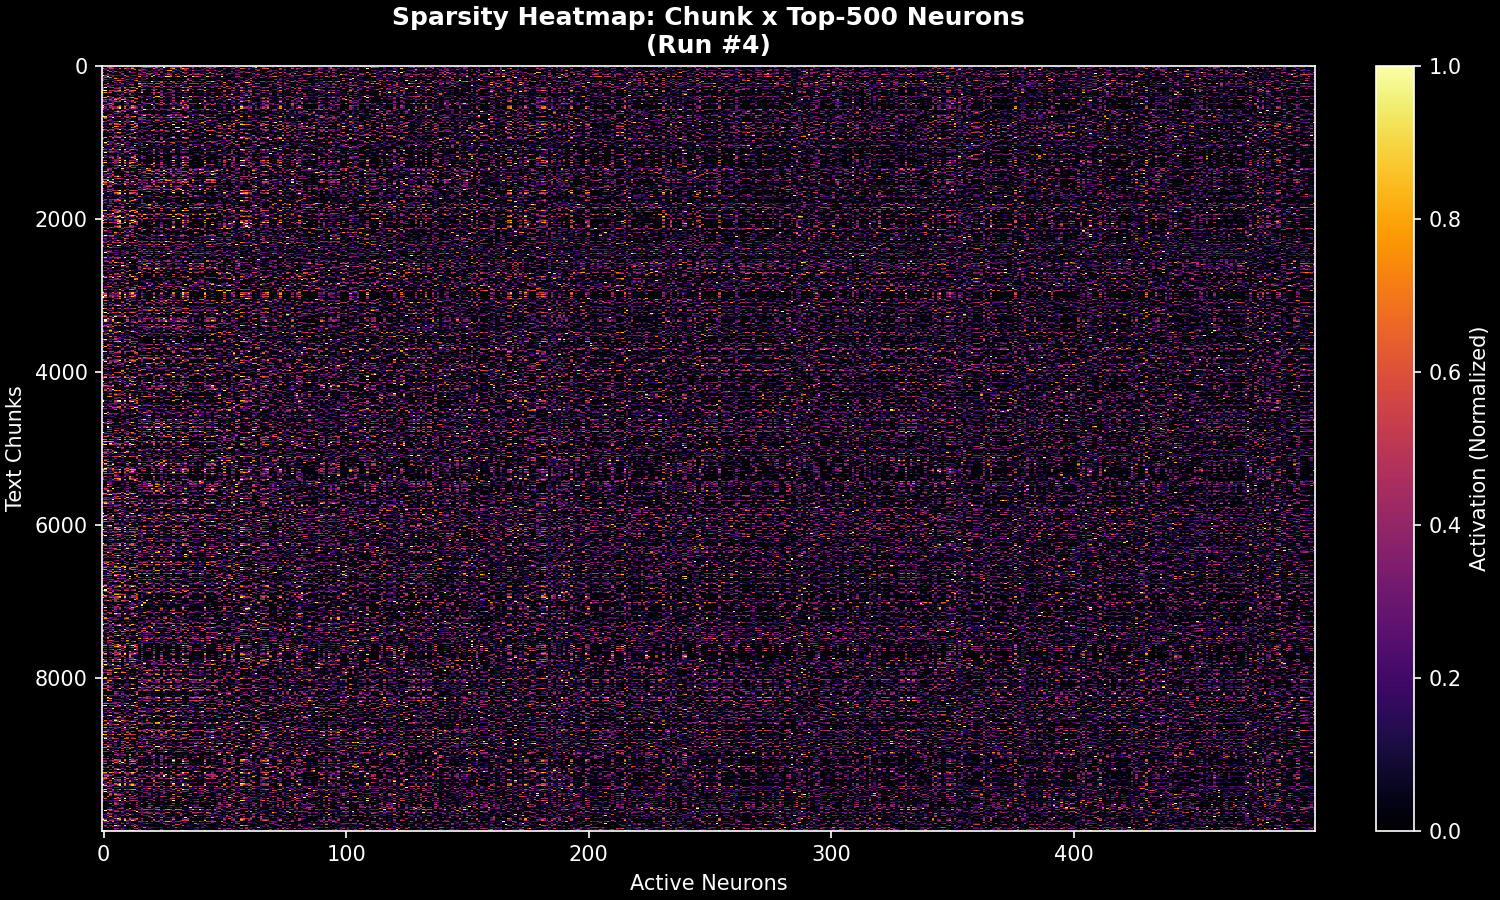
\includegraphics[width=\textwidth]{pictures/latent_matrix.png}

            \vspace{0.2cm}
            {\scriptsize Matrice sparsa $H$ (500 neuroni).\\Poche feature attive per documento\\$\Rightarrow$ \textbf{monosemanticit\`a}.}
        \end{column}
    \end{columns}
\end{frame}

% ============================================================
% SLIDE 13 — Interpretabilit\`a automatica
% ============================================================
\begin{frame}{Interpretabilit\`a automatica: l'LLM Interpreter}
    \centering
    \begin{tikzpicture}[
        scale=0.85,
        arrow/.style={->, thick, >=stealth}
    ]
        % Step 1: Feature si attiva
        \node[draw=gray!50, rectangle, rounded corners=4pt, minimum width=2.5cm, minimum height=1.2cm, align=center, font=\small, fill=green!25!black, text=white] (neuron) at (0, 0) {\textbf{Feature $h_i$}\\si attiva};

        % Step 2: Top-5 documenti + contro-esempi
        \node[draw=gray!50, rectangle, rounded corners=4pt, minimum width=2.8cm, minimum height=1.2cm, align=center, font=\small, fill=blue!25!black, text=white] (docs) at (4.5, 0) {\textbf{Top-5 testi}\\+ contro-esempi};

        % Step 3: LLM Interpreter
        \node[draw=gray!50, rectangle, rounded corners=4pt, minimum width=2.8cm, minimum height=1.2cm, align=center, font=\small, fill=orange!25!black, text=white] (llm) at (9, 0) {\textbf{LLM Interpreter}\\``Cosa hanno in comune?''};

        % Step 4: Etichetta
        \node[draw=gray!50, rectangle, rounded corners=4pt, minimum width=2.5cm, minimum height=1.2cm, align=center, font=\small, fill=violet!25!black, text=white] (label) at (13, 0) {\textbf{Etichetta}\\semantica};

        % Frecce
        \draw[arrow, white] (neuron) -- (docs);
        \draw[arrow, white] (docs) -- (llm);
        \draw[arrow, white] (llm) -- (label);

        % Esempio sotto
        \node[font=\scriptsize, gray!60, text width=2.5cm, align=center] at (0, -1.5) {$h_{42} > 0$};
        \node[font=\scriptsize, gray!60, text width=2.8cm, align=center] at (4.5, -1.5) {``dark matter halo...''\\``galaxy rotation...''\\``WIMP detection...''};
        \node[font=\scriptsize, gray!60, text width=3cm, align=center] at (9, -1.5) {Osserva testi attivanti\\e non attivanti,\\genera un'etichetta};
        \node[font=\scriptsize, gray!60, text width=2.5cm, align=center] at (13, -1.5) {\textbf{``Dark matter\\detection''}};
    \end{tikzpicture}

    \vspace{0.4cm}
    Per \textbf{generalizzare} questo processo e renderlo accessibile, ho costruito una \textbf{web app}.
\end{frame}

% ============================================================
% SLIDE 14 — PRISMA: l'applicazione
% ============================================================
\begin{frame}{PRISMA: l'applicazione}
    \centering
    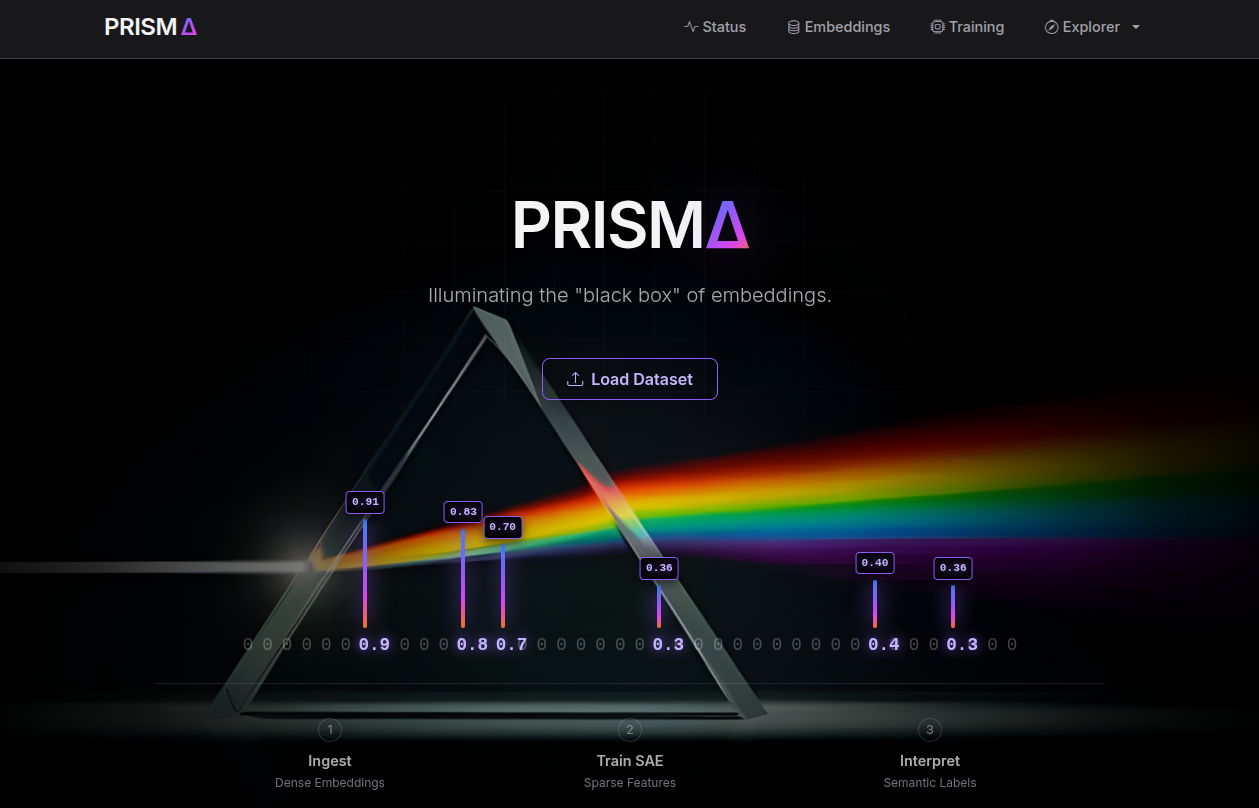
\includegraphics[width=0.85\textwidth]{cap5/home.png}

    \vspace{0.3cm}
    {\small Un'applicazione web che permette di addestrare SAE, esplorare le feature estratte e ottenere le etichette semantiche in modo interattivo.}
\end{frame}

% ============================================================
% SLIDE 15 — La metrica e il futuro
% ============================================================
\begin{frame}{La metrica: Effective Rank}
    \begin{columns}
        \begin{column}{0.5\textwidth}
            \textbf{Idea:} i concetti estratti non sono indipendenti.

            \vspace{0.2cm}
            Es: ``febbre'' e ``polmonite'' si attivano insieme.

            \vspace{0.3cm}
            \textbf{Effective Rank:}
            \[
                ER(H) = \exp\!\left(-\sum_i p_i \log p_i\right)
            \]
            con $p_i = \sigma_i / \|\sigma\|_1$

            \vspace{0.3cm}
            \textbf{Semantic Compression Ratio:}
            \[
                SCR = 100 \cdot \frac{ER_{\text{null}} - ER_{\text{real}}}{ER_{\text{null}}}
            \]


        \end{column}
        \begin{column}{0.45\textwidth}
            \centering
            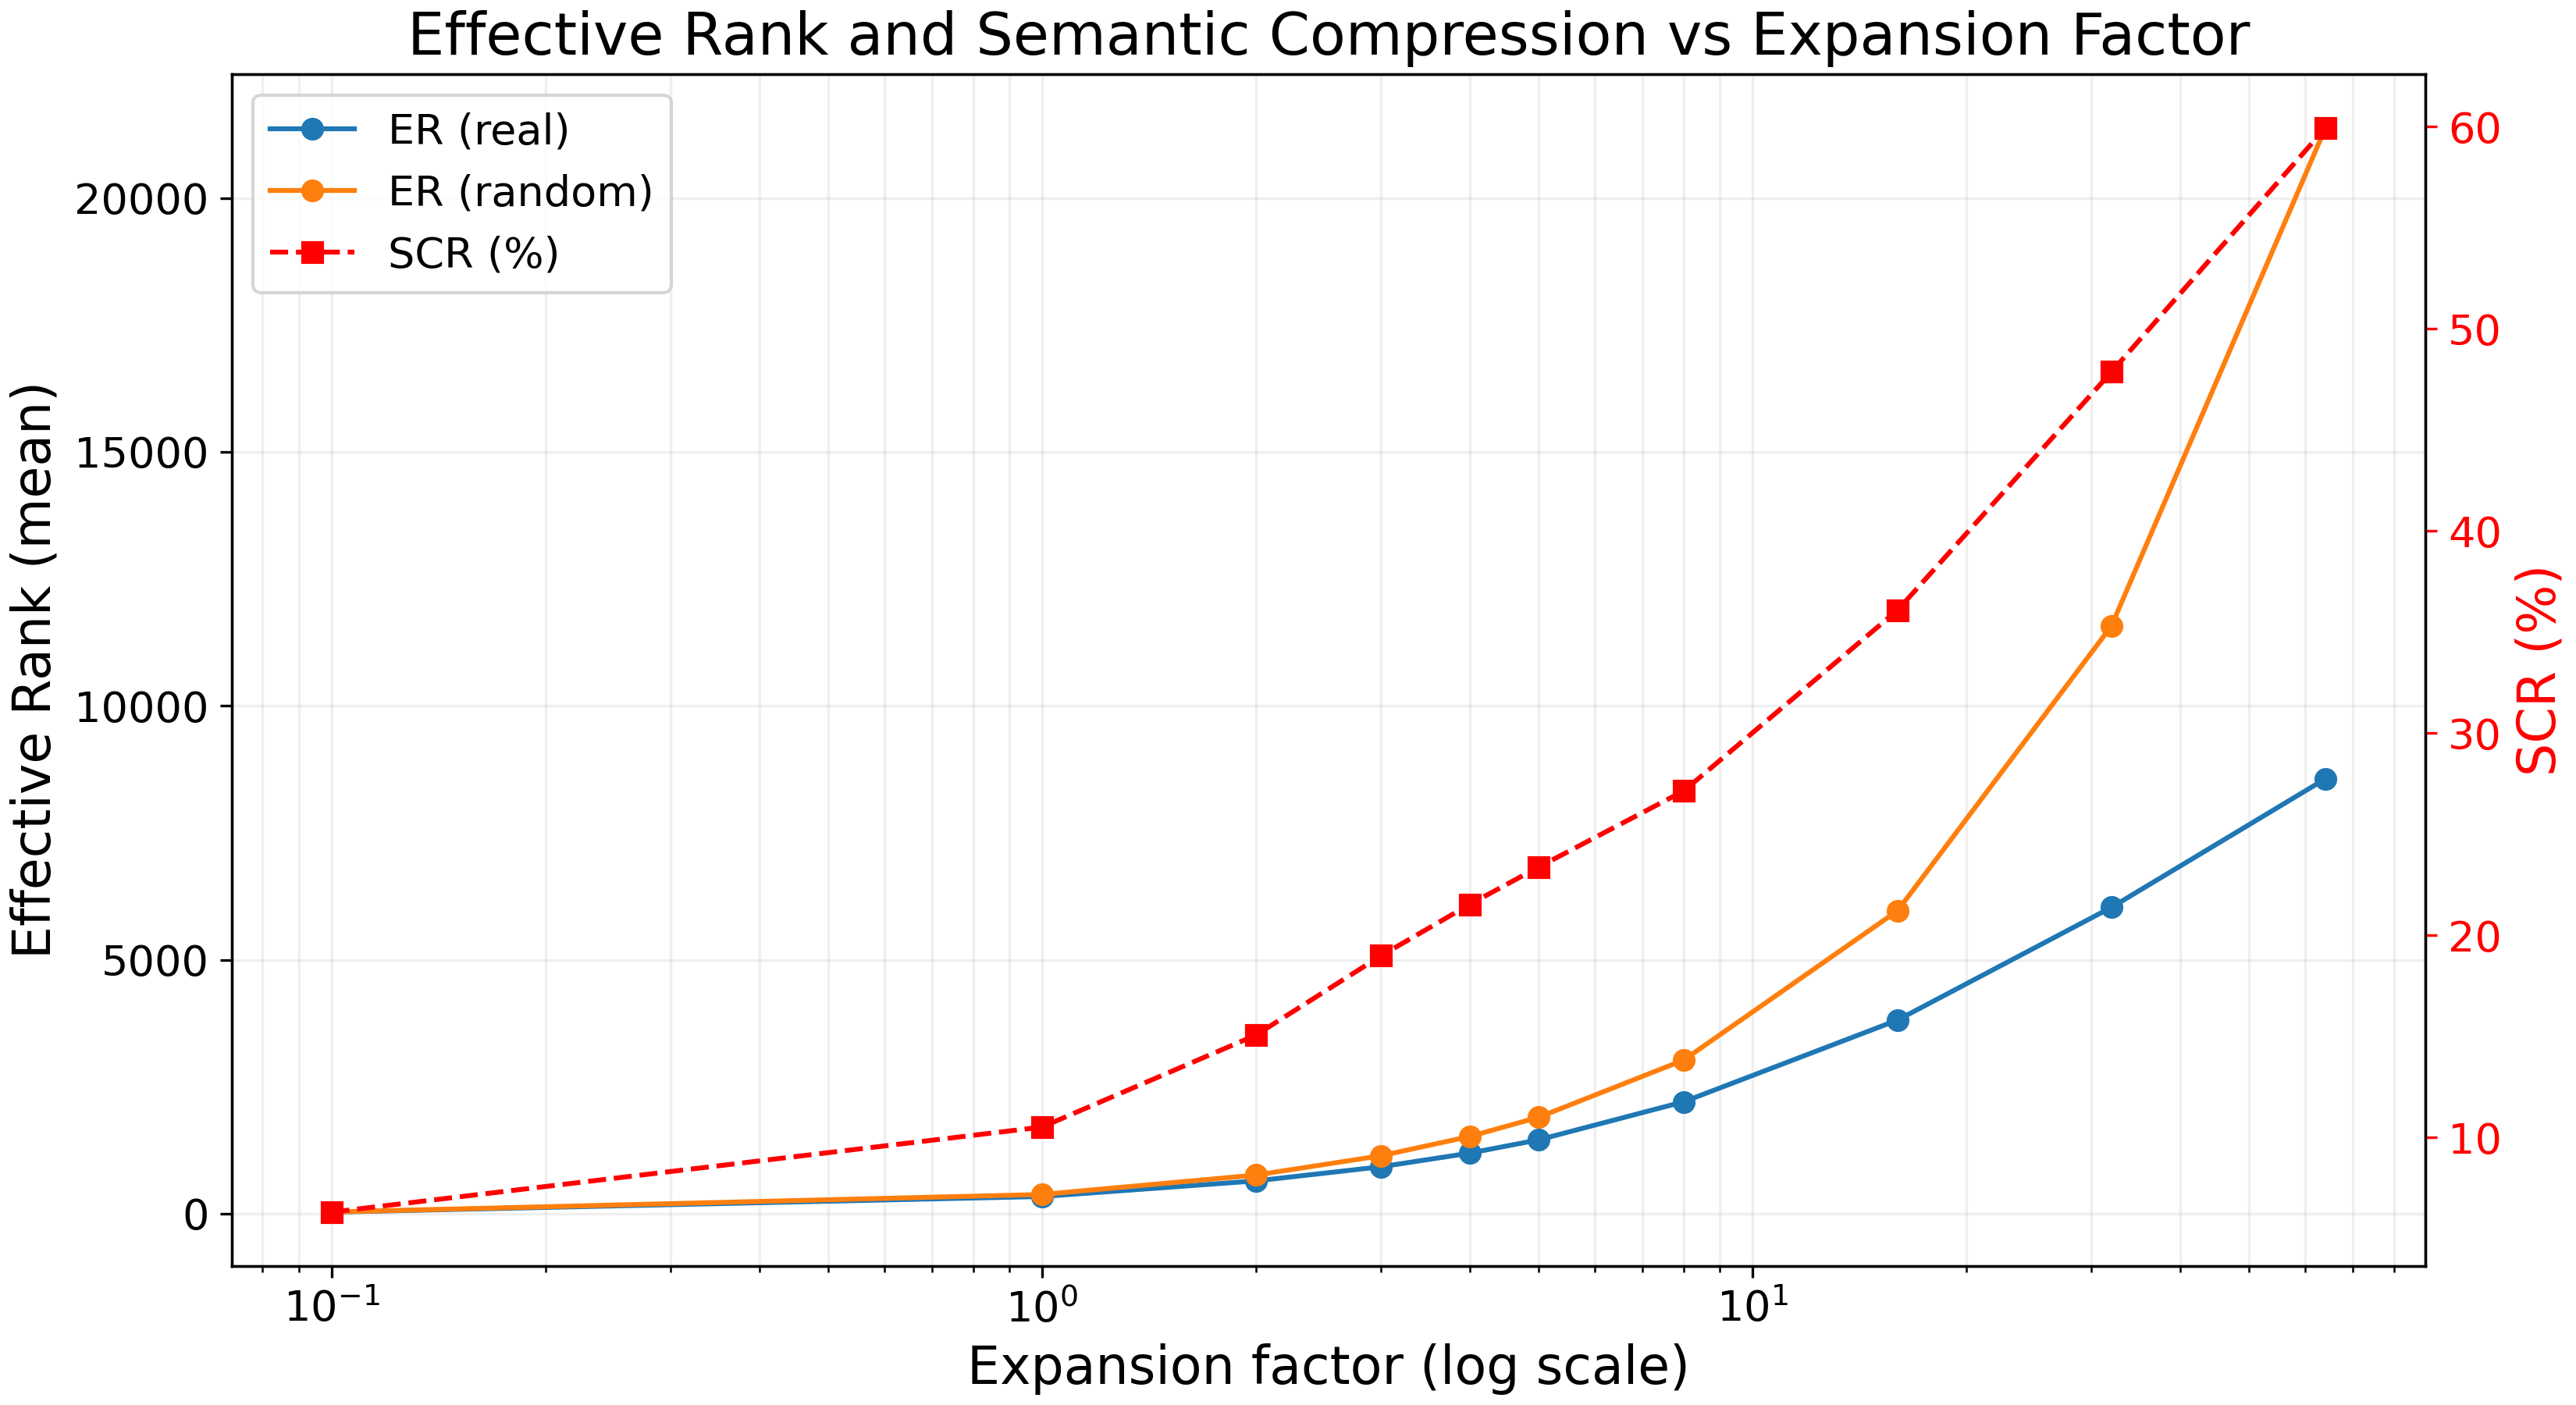
\includegraphics[width=\textwidth]{erank_scr_twinaxis_scr_red.png}

            \vspace{0.2cm}
            {\scriptsize ER vs expansion factor\\(dati reali vs ipotesi nulla)}
        \end{column}
    \end{columns}
\end{frame}

% ============================================================
% SLIDE — Sviluppi futuri
% ============================================================
\begin{frame}{Sviluppi futuri: esistono invarianti semantici?}
    \begin{columns}[T]
        % --- Colonna sinistra: Einstein ---
        \begin{column}{0.42\textwidth}
            \centering
            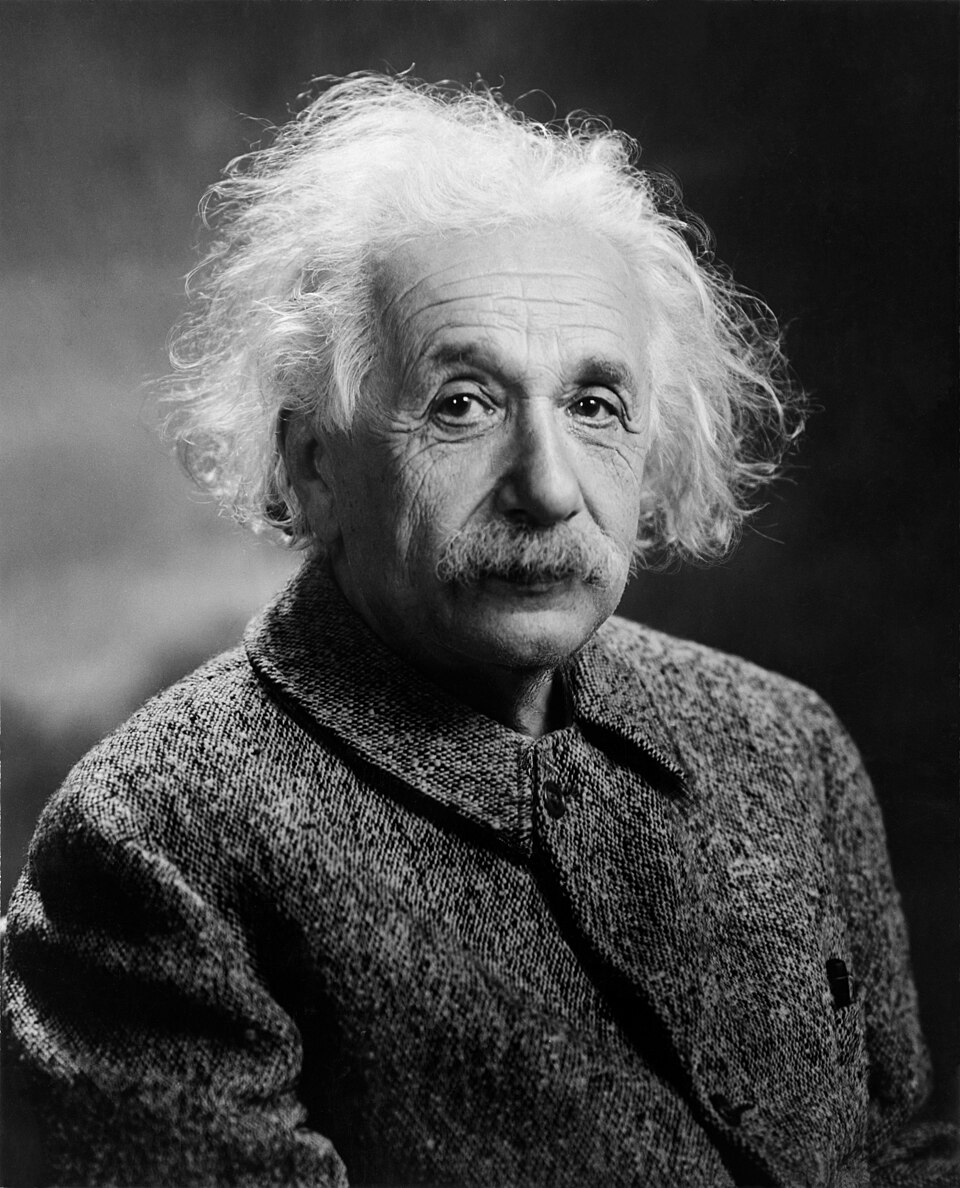
\includegraphics[
                width=\textwidth,
                height=5.5cm,
                keepaspectratio
            ]{pictures/einstein.jpeg}
            \vspace{0.15cm}
            {\scriptsize\color{gray!60}\\
            Relatività: alcune quantità non dipendono dal sistema di riferimento.}
        \end{column}
        % --- Colonna destra: contenuto concettuale ---
        \begin{column}{0.55\textwidth}
            \small
            \begin{block}{}
                \centering
                \large
                La velocità della luce \(c\) è \textbf{invariante}
            \end{block}
            \vspace{0.2cm}
            Le coordinate cambiano, il sistema di riferimento cambia, ma alcune quantità restano le stesse.\\
            \textbf{Domanda analoga:} se cambiamo rappresentazione, esistono quantità semantiche che restano \textbf{invarianti}?

            \vspace{0.2cm}
            \centering
            \begin{tikzpicture}[scale=0.7, transform shape, every node/.style={text=white}]
                \node[draw=red!60, fill=red!30!black, rounded corners, minimum width=2.2cm, minimum height=0.7cm, font=\small] (dense) at (0, 3) {Densa};
                \node[draw=cyan!60, fill=cyan!30!black, rounded corners, minimum width=2.2cm, minimum height=0.7cm, font=\small] (sparse) at (0, 1.5) {Sparsa};
                \node[draw=green!60, fill=green!30!black, rounded corners, minimum width=2.2cm, minimum height=0.7cm, font=\small] (human) at (0, 0) {Umana};
                \node[draw=yellow!60, fill=yellow!30!black, rounded corners, minimum width=2.2cm, minimum height=1cm, font=\small, align=center] (inv) at (3.5, 1.5) {Invarianti\\semantici\\$ds^2_{\text{sem}}$?};
                \draw[->, thick, red!60] (dense.east) -- (inv.north west);
                \draw[->, thick, cyan!60] (sparse.east) -- (inv.west);
                \draw[->, thick, green!60] (human.east) -- (inv.south west);
            \end{tikzpicture}
        \end{column}
    \end{columns}
\end{frame}

% ============================================================
% SLIDE FINALE — Grazie
% ============================================================
\begin{frame}[plain]
    \centering
    \vspace{1.5cm}

    % Grazie con rainbow
    \begin{tikzpicture}
        \node[inner sep=0pt] (g) {\phantom{\fontsize{40}{48}\selectfont\bfseries Grazie}};
        \shade[left color=red, right color=violet, middle color=green!80!yellow]
            (g.south west) rectangle (g.north east);
        \node[inner sep=0pt, text=white] at (g.center) {\fontsize{40}{48}\selectfont\bfseries Grazie};
    \end{tikzpicture}

    \vspace{0.8cm}
    {\large\color{white} Edoardo Tedesco}

    \vspace{0.3cm}
    {\small\color{gray!60} Corso di Laurea Magistrale in Fisica\\
    Universit\`a degli Studi di Milano}

    \vspace{0.5cm}
    {\small\color{gray!50}
    Relatore esterno: Prof. Mirko Cesarini\\
    Relatore interno: Prof. Marco Gherardi}
\end{frame}


% ============================================================
% SLIDE BACKUP — Platonic Representation Hypothesis
% ============================================================
\begin{frame}{Platonic Representation Hypothesis}
    \begin{columns}[T]
        \begin{column}{0.45\textwidth}
            \centering
            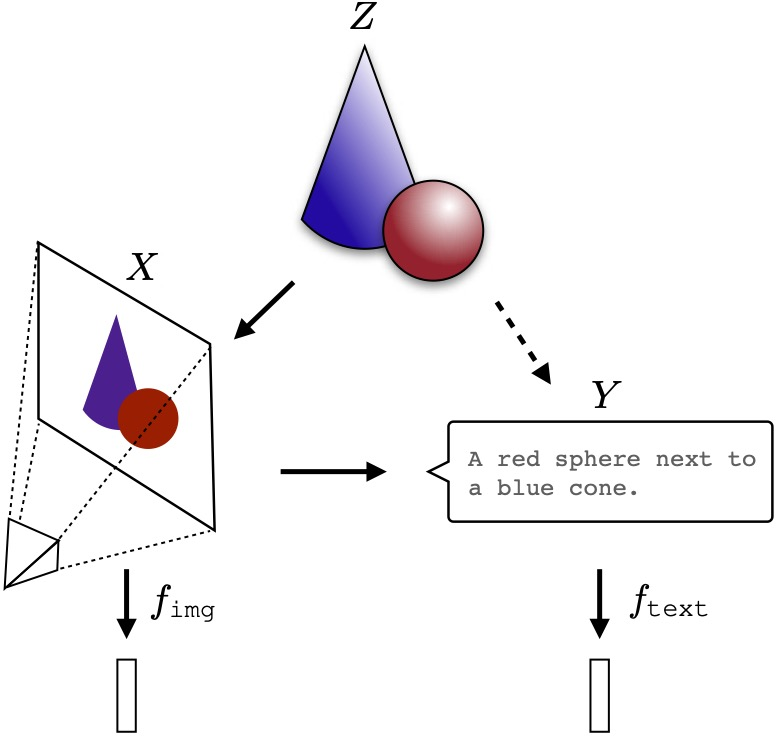
\includegraphics[
                width=\textwidth,
                height=6cm,
                keepaspectratio
            ]{pictures/platonic_rep_less_space_v2.jpg}

            \vspace{0.2cm}
            {\tiny Huh, Cheung, Wang, Isola (2024)}
        \end{column}
        \begin{column}{0.52\textwidth}
            Un evento reale $Z$ può essere osservato attraverso modalità diverse:

            \vspace{0.2cm}
            \begin{itemize}
                \item \textbf{Immagine} $X$ $\xrightarrow{f_{\text{img}}}$ embedding visivo
                \item \textbf{Testo} $Y$ $\xrightarrow{f_{\text{text}}}$ embedding linguistico
            \end{itemize}

            \vspace{0.3cm}
            \textbf{Ipotesi:} al crescere della scala, le rappresentazioni apprese da modelli diversi \textbf{convergono} verso uno stesso modello statistico della realtà.

            \vspace{0.3cm}
            Come la \textit{realtà ideale} di Platone: esiste una rappresentazione sottostante, indipendente dalla modalità.

            \vspace{0.3cm}


            \vspace{0.2cm}
            {\small\color{gray!60} Modelli più grandi misurano le distanze tra dati in modo sempre più simile, indipendentemente dalla modalità.}
        \end{column}
    \end{columns}
\end{frame}

% ============================================================
% SLIDE BACKUP — Il Mito della Caverna
% ============================================================
\begin{frame}{Il Mito della Caverna di Platone}
    \begin{columns}[T]
        \begin{column}{0.48\textwidth}
            \centering
            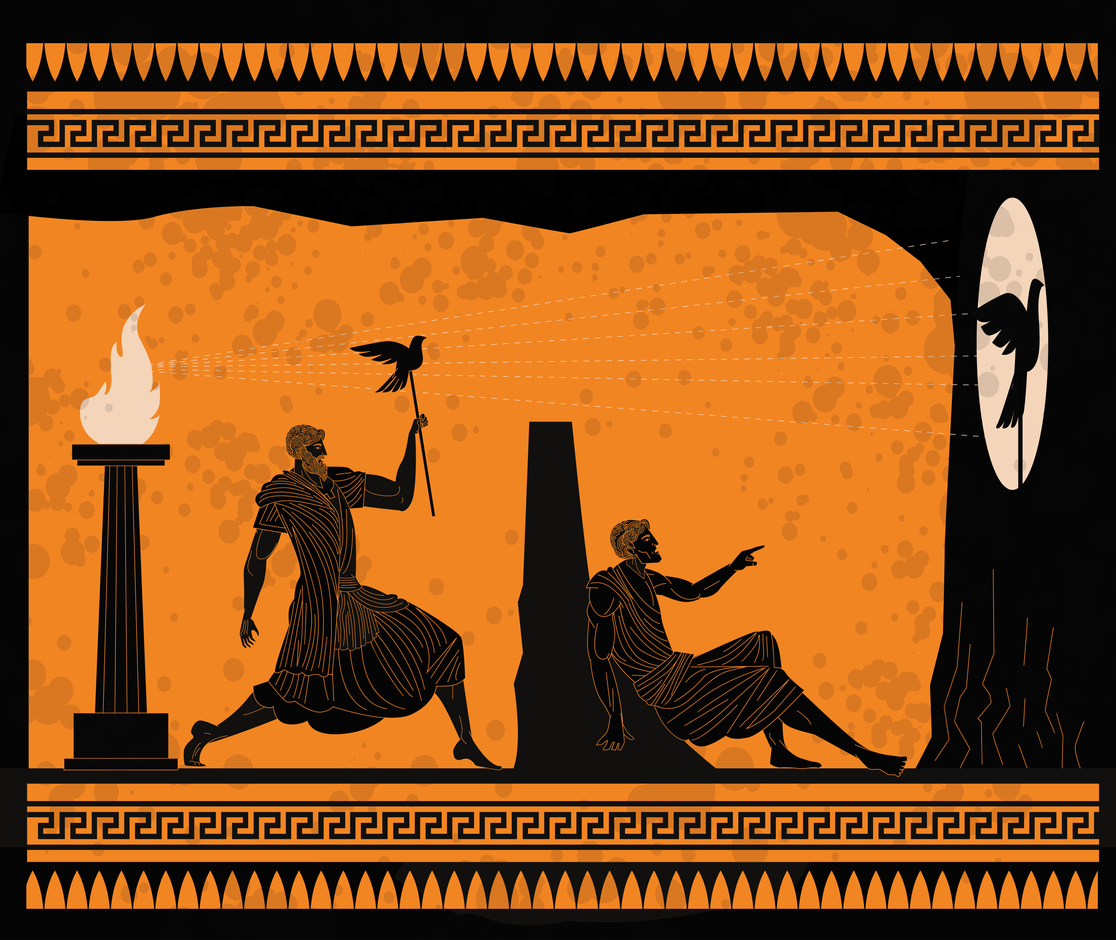
\includegraphics[
                width=\textwidth,
                height=6.5cm,
                keepaspectratio
            ]{pictures/mito_caverna.jpeg}
        \end{column}
        \begin{column}{0.48\textwidth}
            I prigionieri vedono solo \textbf{ombre} proiettate sulla parete della caverna.
            \vspace{0.3cm}
            \begin{block}{}
                \centering
                Le ombre sono diverse,\\ma l'oggetto è \textbf{lo stesso}.
            \end{block}

            \vspace{0.3cm}
            L'ipotesi platonica suggerisce che i modelli di AI, al crescere della scala, stiano \textbf{uscendo dalla caverna}: convergono verso la stessa rappresentazione della realtà.

            \vspace{0.3cm}
            \centering
            \begin{tikzpicture}[scale=0.6, transform shape, every node/.style={text=white}]
                \node[draw=orange!60, fill=orange!25!black, rounded corners, font=\small] (real) at (0, 0) {Realtà $Z$};
                \node[draw=red!50, fill=red!20!black, rounded corners, font=\scriptsize] (img) at (-2.5, -1.5) {Ombra: immagine};
                \node[draw=cyan!50, fill=cyan!20!black, rounded corners, font=\scriptsize] (txt) at (2.5, -1.5) {Ombra: testo};
                \draw[->, thick, red!50] (real) -- (img);
                \draw[->, thick, cyan!50] (real) -- (txt);
            \end{tikzpicture}
        \end{column}
    \end{columns}
\end{frame}



% ============================================================
% SLIDE BACKUP — Hubble Deep Field e PRISMA
% ============================================================
\begin{frame}{Il Deep Field di Hubble (1996)}
    \begin{columns}[T]
        \begin{column}{0.45\textwidth}
            \centering
            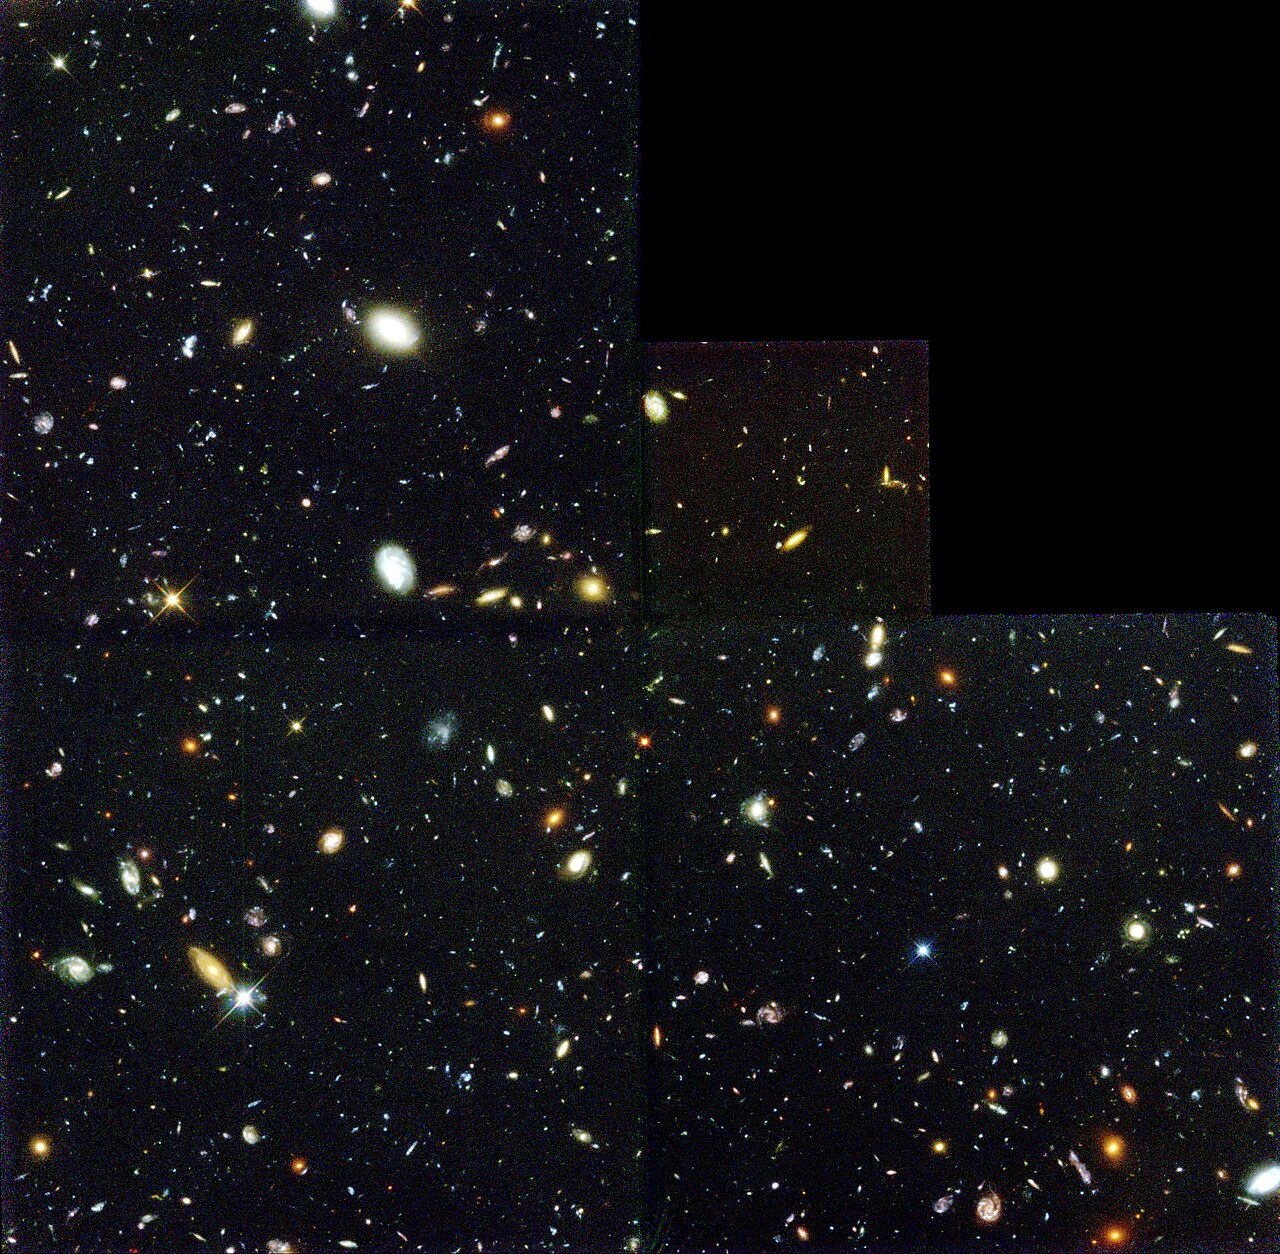
\includegraphics[
                width=\textwidth,
                height=6.5cm,
                keepaspectratio
            ]{pictures/hubble.jpg}

            \vspace{0.15cm}
            {\tiny Hubble Deep Field, NASA/STScI, 1996}
        \end{column}
        \begin{column}{0.52\textwidth}
            Nel 1995, Hubble puntò verso una zona di cielo apparentemente \textbf{vuota} per 10 giorni consecutivi nelle notti tra il 18 e il 28 dicembre.

            \vspace{0.3cm}
            
            
            Il risultato: \textbf{oltre 3000 galassie} nascoste in un'area grande quanto un granello di sabbia a braccia tese.


\vspace{0.3cm}
            Potremmo trovare una struttura nascosta nel profondo dell'\textbf{universo semantico}.



        \end{column}
    \end{columns}
\end{frame}

% ============================================================
% SLIDE BACKUP — Feature Families: le matrici
% ============================================================
\begin{frame}{Feature Families --- le matrici}
    \textbf{Matrice delle attivazioni} $H \in \mathbb{R}^{N \times n}$\quad (documenti $\times$ feature):
    \[
        H_{ki} = \left[ f_\theta(\mathbf{x}_k) \right]_i
    \]

    \vspace{0.2cm}
    \textbf{Matrice binaria} $A \in \{0,1\}^{N \times n}$:
    \[
        A_{ki} = \begin{cases} 1 & \text{se } H_{ki} > 0 \\ 0 & \text{altrimenti} \end{cases}
    \]

    \vspace{0.2cm}
    \begin{columns}
        \begin{column}{0.48\textwidth}
            \textbf{Co-occorrenza} $C = A^T A$:
            \[
                C_{ij} = \sum_{k=1}^{N} A_{ki} \cdot A_{kj}
            \]
            {\small Quanti documenti attivano \textit{entrambe} le feature $i$ e $j$.}
        \end{column}
        \begin{column}{0.48\textwidth}
            \textbf{Similarit\`a attivazioni} $D = H^T H$:
            \[
                D_{ij} = \sum_{k=1}^{N} H_{ki} \cdot H_{kj}
            \]
            {\small Come $C$, ma pesata per \textbf{intensit\`a}.}
        \end{column}
    \end{columns}
\end{frame}

% ============================================================
% SLIDE BACKUP — Similarità geometrica e normalizzazione
% ============================================================
\begin{frame}{Similarit\`a geometrica $S$ e $C^{\text{norm}}$}
    \begin{columns}[T]
        \begin{column}{0.46\textwidth}
            \textbf{Similarit\`a geometrica} $S$:
            {\small\[
                S_{ij} = \frac{\mathbf{w}_i^T \mathbf{w}_j}{\|\mathbf{w}_i\| \|\mathbf{w}_j\|} = \cos\theta_{ij}
            \]}

            {\small $\mathbf{w}_i$ = colonna $i$ del decoder $W_d$.}

            \vspace{0.2cm}
            {\small Le colonne del decoder sono le \textbf{direzioni semantiche} nello spazio degli embedding.}

            \vspace{0.2cm}
            {\small $S_{ij} \approx 1$ $\Rightarrow$ le feature ``puntano'' nella stessa direzione.}
        \end{column}
        \begin{column}{0.46\textwidth}
            \textbf{Co-occorrenza normalizzata}:
            \[
                C^{\text{norm}}_{ij} = \frac{C_{ij}}{f_i + \epsilon}
            \]
            con $f_i = C_{ii} = \sum_k A_{ki}$ (frequenza).

            \vspace{0.3cm}
            {\small Frazione delle attivazioni di $i$ in cui anche $j$ \`e attiva.}

            \vspace{0.2cm}
            {\small \textbf{Non simmetrica:} $C^{\text{norm}}_{ij} \neq C^{\text{norm}}_{ji}$}

            \vspace{0.2cm}
            {\small Es: ``Ising model'' co-occorre con ``Phase Transitions'', ma non viceversa.}
        \end{column}
    \end{columns}
\end{frame}

% ============================================================
% SLIDE BACKUP — Algoritmo Feature Families
% ============================================================
\begin{frame}{Algoritmo delle Feature Families}
    \begin{enumerate}
 

        \item \textbf{Costruzione grafo pesato}: soglia $\tau = 0.1$ su $C^{\text{norm}}$
        \[
            \text{arco } (i,j) \iff C^{\text{norm}}_{ij} > \tau
        \]
        con peso $w_{ij} = C^{\text{norm}}_{ij}$

        \item \textbf{Maximum Spanning Tree}: albero che massimizza la somma dei pesi (relazioni pi\`u forti), senza cicli

        \item \textbf{Orientamento archi}: dal pi\`u frequente al meno frequente
        \[
            i \to j \quad \iff \quad f_i > f_j
        \]
        {\small Intuizione: concetti generali $\to$ concetti specifici (parent $\to$ child)}

        \item \textbf{Estrazione famiglie}: radici (nodi senza archi entranti). Ogni albero = una famiglia.

    \end{enumerate}

    \vspace{0.2cm}
    \centering
    {\small\color{gray!60} Risultato: \textbf{590 feature families} con topologia a stella (parent $\to$ children).}
\end{frame}

% ============================================================
% SLIDE BACKUP — Feature Splitting vs Feature Families
% ============================================================
\begin{frame}{Feature Splitting vs Feature Families}
    \begin{columns}
        \begin{column}{0.48\textwidth}
            \textbf{Feature Splitting}\\
            {\small (tra SAE diversi)}

            \vspace{0.3cm}
            Si usa la matrice $S$ per confrontare feature \textit{tra} due SAE con expansion factor diversi.

            \vspace{0.2cm}
            Per ogni feature $j$ del SAE grande:
            \[
                i^*(j) = \underset{i}{\mathrm{arg\,max}} \; S_{ij}
            \]

            \vspace{0.2cm}
            \begin{itemize}
                \item $S^*_j > 0.95$ $\to$ \textbf{ricorrente}
                \item $0.5 < S^*_j < 0.95$ $\to$ \textbf{splitting}
                \item $S^*_j < 0.5$ $\to$ \textbf{nuova}
            \end{itemize}
        \end{column}
        \begin{column}{0.48\textwidth}
            \textbf{Feature Families}\\
            {\small (dentro un singolo SAE)}

            \vspace{0.3cm}
            Si usa $C^{\text{norm}}$ per trovare gerarchie \textit{dentro} lo stesso SAE.

            \vspace{0.2cm}
            Topologia a stella:

            \vspace{0.2cm}
            \begin{tikzpicture}[scale=0.6, transform shape, every node/.style={text=white}]
                \node[draw=cyan!60, circle, fill=cyan!30!black, minimum size=0.8cm, font=\scriptsize] (p) at (0, 0) {Parent};
                \node[draw=violet!60, circle, fill=violet!30!black, minimum size=0.6cm, font=\tiny] (c1) at (-1.5, -1.5) {C1};
                \node[draw=violet!60, circle, fill=violet!30!black, minimum size=0.6cm, font=\tiny] (c2) at (0, -1.8) {C2};
                \node[draw=violet!60, circle, fill=violet!30!black, minimum size=0.6cm, font=\tiny] (c3) at (1.5, -1.5) {C3};
                \draw[->, thick, gray!60] (p) -- (c1);
                \draw[->, thick, gray!60] (p) -- (c2);
                \draw[->, thick, gray!60] (p) -- (c3);
            \end{tikzpicture}

            \vspace{0.2cm}
            {\small Es: ``Time in physics'' $\to$ 47 children (Time Reversal, Quantum Clocks, ...)}
        \end{column}
    \end{columns}
\end{frame}

\end{document}
